\documentclass[twoside]{book}

% Packages required by doxygen
\usepackage{fixltx2e}
\usepackage{calc}
\usepackage{doxygen}
\usepackage[export]{adjustbox} % also loads graphicx
\usepackage{graphicx}
\usepackage[utf8]{inputenc}
\usepackage{makeidx}
\usepackage{multicol}
\usepackage{multirow}
\PassOptionsToPackage{warn}{textcomp}
\usepackage{textcomp}
\usepackage[nointegrals]{wasysym}
\usepackage[table]{xcolor}

% Font selection
\usepackage[T1]{fontenc}
\usepackage[scaled=.90]{helvet}
\usepackage{courier}
\usepackage{amssymb}
\usepackage{sectsty}
\renewcommand{\familydefault}{\sfdefault}
\allsectionsfont{%
  \fontseries{bc}\selectfont%
  \color{darkgray}%
}
\renewcommand{\DoxyLabelFont}{%
  \fontseries{bc}\selectfont%
  \color{darkgray}%
}
\newcommand{\+}{\discretionary{\mbox{\scriptsize$\hookleftarrow$}}{}{}}

% Page & text layout
\usepackage{geometry}
\geometry{%
  a4paper,%
  top=2.5cm,%
  bottom=2.5cm,%
  left=2.5cm,%
  right=2.5cm%
}
\tolerance=750
\hfuzz=15pt
\hbadness=750
\setlength{\emergencystretch}{15pt}
\setlength{\parindent}{0cm}
\setlength{\parskip}{3ex plus 2ex minus 2ex}
\makeatletter
\renewcommand{\paragraph}{%
  \@startsection{paragraph}{4}{0ex}{-1.0ex}{1.0ex}{%
    \normalfont\normalsize\bfseries\SS@parafont%
  }%
}
\renewcommand{\subparagraph}{%
  \@startsection{subparagraph}{5}{0ex}{-1.0ex}{1.0ex}{%
    \normalfont\normalsize\bfseries\SS@subparafont%
  }%
}
\makeatother

% Headers & footers
\usepackage{fancyhdr}
\pagestyle{fancyplain}
\fancyhead[LE]{\fancyplain{}{\bfseries\thepage}}
\fancyhead[CE]{\fancyplain{}{}}
\fancyhead[RE]{\fancyplain{}{\bfseries\leftmark}}
\fancyhead[LO]{\fancyplain{}{\bfseries\rightmark}}
\fancyhead[CO]{\fancyplain{}{}}
\fancyhead[RO]{\fancyplain{}{\bfseries\thepage}}
\fancyfoot[LE]{\fancyplain{}{}}
\fancyfoot[CE]{\fancyplain{}{}}
\fancyfoot[RE]{\fancyplain{}{\bfseries\scriptsize Generated by Doxygen }}
\fancyfoot[LO]{\fancyplain{}{\bfseries\scriptsize Generated by Doxygen }}
\fancyfoot[CO]{\fancyplain{}{}}
\fancyfoot[RO]{\fancyplain{}{}}
\renewcommand{\footrulewidth}{0.4pt}
\renewcommand{\chaptermark}[1]{%
  \markboth{#1}{}%
}
\renewcommand{\sectionmark}[1]{%
  \markright{\thesection\ #1}%
}

% Indices & bibliography
\usepackage{natbib}
\usepackage[titles]{tocloft}
\setcounter{tocdepth}{3}
\setcounter{secnumdepth}{5}
\makeindex

% Hyperlinks (required, but should be loaded last)
\usepackage{ifpdf}
\ifpdf
  \usepackage[pdftex,pagebackref=true]{hyperref}
\else
  \usepackage[ps2pdf,pagebackref=true]{hyperref}
\fi
\hypersetup{%
  colorlinks=true,%
  linkcolor=blue,%
  citecolor=blue,%
  unicode%
}

% Custom commands
\newcommand{\clearemptydoublepage}{%
  \newpage{\pagestyle{empty}\cleardoublepage}%
}

\usepackage{caption}
\captionsetup{labelsep=space,justification=centering,font={bf},singlelinecheck=off,skip=4pt,position=top}

%===== C O N T E N T S =====

\begin{document}

% Titlepage & ToC
\hypersetup{pageanchor=false,
             bookmarksnumbered=true,
             pdfencoding=unicode
            }
\pagenumbering{alph}
\begin{titlepage}
\vspace*{7cm}
\begin{center}%
{\Large Exo\+Spec }\\
\vspace*{1cm}
{\large Generated by Doxygen 1.8.13}\\
\end{center}
\end{titlepage}
\clearemptydoublepage
\pagenumbering{roman}
\tableofcontents
\clearemptydoublepage
\pagenumbering{arabic}
\hypersetup{pageanchor=true}

%--- Begin generated contents ---
\chapter{Hierarchical Index}
\section{Class Hierarchy}
This inheritance list is sorted roughly, but not completely, alphabetically\+:\begin{DoxyCompactList}
\item Exception\begin{DoxyCompactList}
\item \contentsline{section}{exospec.\+lc\+\_\+class.\+Different\+File\+Sizes}{\pageref{classexospec_1_1lc__class_1_1_different_file_sizes}}{}
\item \contentsline{section}{exospec.\+lc\+\_\+class.\+Different\+Param\+Num}{\pageref{classexospec_1_1lc__class_1_1_different_param_num}}{}
\item \contentsline{section}{exospec.\+lc\+\_\+class.\+Empty\+File}{\pageref{classexospec_1_1lc__class_1_1_empty_file}}{}
\item \contentsline{section}{exospec.\+lc\+\_\+class.\+Empty\+Folder}{\pageref{classexospec_1_1lc__class_1_1_empty_folder}}{}
\item \contentsline{section}{exospec.\+lc\+\_\+class.\+Incorrect\+Name\+Format}{\pageref{classexospec_1_1lc__class_1_1_incorrect_name_format}}{}
\item \contentsline{section}{exospec.\+read\+\_\+input.\+Empty\+File}{\pageref{classexospec_1_1read__input_1_1_empty_file}}{}
\item \contentsline{section}{exospec.\+read\+\_\+input.\+No\+Input}{\pageref{classexospec_1_1read__input_1_1_no_input}}{}
\end{DoxyCompactList}
\item \contentsline{section}{exospec.\+lc\+\_\+class.\+Light\+Curve}{\pageref{classexospec_1_1lc__class_1_1_light_curve}}{}
\item \contentsline{section}{exospec.\+lc\+\_\+class.\+Light\+Curve\+Data}{\pageref{classexospec_1_1lc__class_1_1_light_curve_data}}{}
\item object\begin{DoxyCompactList}
\item \contentsline{section}{exospec.\+mcmc.\+M\+C\+MC}{\pageref{classexospec_1_1mcmc_1_1_m_c_m_c}}{}
\item \contentsline{section}{exospec.\+Transit\+Model.\+Transit\+Model}{\pageref{classexospec_1_1_transit_model_1_1_transit_model}}{}
\end{DoxyCompactList}
\item \contentsline{section}{exospec.\+read\+\_\+input.\+read\+\_\+input}{\pageref{classexospec_1_1read__input_1_1read__input}}{}
\end{DoxyCompactList}

\chapter{Class Index}
\section{Class List}
Here are the classes, structs, unions and interfaces with brief descriptions\+:\begin{DoxyCompactList}
\item\contentsline{section}{\hyperlink{classexospec_1_1lc__class_1_1_different_file_sizes}{exospec.\+lc\+\_\+class.\+Different\+File\+Sizes} \\*Raise when one the light curve file does not have the same size with light curve file for the lowest wavelength (this file serves as reference) }{\pageref{classexospec_1_1lc__class_1_1_different_file_sizes}}{}
\item\contentsline{section}{\hyperlink{classexospec_1_1lc__class_1_1_different_param_num}{exospec.\+lc\+\_\+class.\+Different\+Param\+Num} \\*Raise when one the light curve file does not have the same number of parameters with light curve file for the lowest wavelength (this file serves as reference) }{\pageref{classexospec_1_1lc__class_1_1_different_param_num}}{}
\item\contentsline{section}{\hyperlink{classexospec_1_1read__input_1_1_empty_file}{exospec.\+read\+\_\+input.\+Empty\+File} \\*Raise exception when the input file is empty or only has comments }{\pageref{classexospec_1_1read__input_1_1_empty_file}}{}
\item\contentsline{section}{\hyperlink{classexospec_1_1lc__class_1_1_empty_file}{exospec.\+lc\+\_\+class.\+Empty\+File} \\*Raise when the light curve file is empty }{\pageref{classexospec_1_1lc__class_1_1_empty_file}}{}
\item\contentsline{section}{\hyperlink{classexospec_1_1lc__class_1_1_empty_folder}{exospec.\+lc\+\_\+class.\+Empty\+Folder} \\*Raise exception when the light curve folder is empty }{\pageref{classexospec_1_1lc__class_1_1_empty_folder}}{}
\item\contentsline{section}{\hyperlink{classexospec_1_1lc__class_1_1_incorrect_name_format}{exospec.\+lc\+\_\+class.\+Incorrect\+Name\+Format} \\*Raise when the light curve file name is not under the expected format sample\+\_\+lc\+\_\+$<$wavelength$>$.\+txt }{\pageref{classexospec_1_1lc__class_1_1_incorrect_name_format}}{}
\item\contentsline{section}{\hyperlink{classexospec_1_1lc__class_1_1_light_curve}{exospec.\+lc\+\_\+class.\+Light\+Curve} \\*List all the light curve files in the indicated folder if the user decided to use another wavelength resolution than the one provided with the files, the code compute the resulting number of new wavelength to be used loop over the light curve files to get their file names and original wavelengths if the user decided to use a new wavelength resolution, the code computes the new wavelength to be used instantiate the new lc objects (with new wave\+\_\+bin\+\_\+size) Warning\+: The code is not able yet to handle situation where files\+\_\+num is not proportional to wave\+\_\+bin\+\_\+size }{\pageref{classexospec_1_1lc__class_1_1_light_curve}}{}
\item\contentsline{section}{\hyperlink{classexospec_1_1lc__class_1_1_light_curve_data}{exospec.\+lc\+\_\+class.\+Light\+Curve\+Data} \\*This class is used by the class \hyperlink{classexospec_1_1lc__class_1_1_light_curve}{Light\+Curve} to extract, store and process the data from the light curve files }{\pageref{classexospec_1_1lc__class_1_1_light_curve_data}}{}
\item\contentsline{section}{\hyperlink{classexospec_1_1mcmc_1_1_m_c_m_c}{exospec.\+mcmc.\+M\+C\+MC} \\*Class to run \hyperlink{classexospec_1_1mcmc_1_1_m_c_m_c}{M\+C\+MC} to fit curve and produce diagnostic plots and statistics Uses emcee (to run \hyperlink{classexospec_1_1mcmc_1_1_m_c_m_c}{M\+C\+MC}) and corner (to produce triangle plots) }{\pageref{classexospec_1_1mcmc_1_1_m_c_m_c}}{}
\item\contentsline{section}{\hyperlink{classexospec_1_1read__input_1_1_no_input}{exospec.\+read\+\_\+input.\+No\+Input} \\*Raise exception when the input entry is not properly set }{\pageref{classexospec_1_1read__input_1_1_no_input}}{}
\item\contentsline{section}{\hyperlink{classexospec_1_1read__input_1_1read__input}{exospec.\+read\+\_\+input.\+read\+\_\+input} \\*Reads the input file and stores the input entries }{\pageref{classexospec_1_1read__input_1_1read__input}}{}
\item\contentsline{section}{\hyperlink{classexospec_1_1_transit_model_1_1_transit_model}{exospec.\+Transit\+Model.\+Transit\+Model} \\*Class to estimate the Transit Model with the customized kernel }{\pageref{classexospec_1_1_transit_model_1_1_transit_model}}{}
\end{DoxyCompactList}

\chapter{Class Documentation}
\hypertarget{classexospec_1_1lc__class_1_1_different_file_sizes}{}\section{exospec.\+lc\+\_\+class.\+Different\+File\+Sizes Class Reference}
\label{classexospec_1_1lc__class_1_1_different_file_sizes}\index{exospec.\+lc\+\_\+class.\+Different\+File\+Sizes@{exospec.\+lc\+\_\+class.\+Different\+File\+Sizes}}
Inheritance diagram for exospec.\+lc\+\_\+class.\+Different\+File\+Sizes\+:\begin{figure}[H]
\begin{center}
\leavevmode
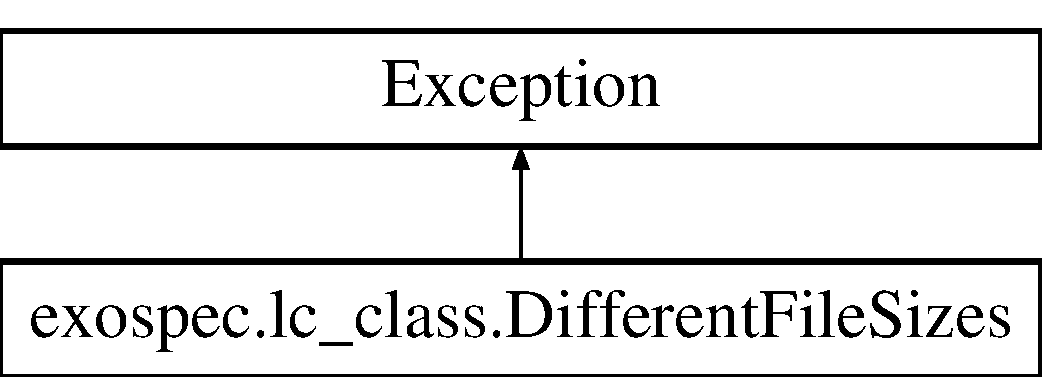
\includegraphics[height=2.000000cm]{classexospec_1_1lc__class_1_1_different_file_sizes}
\end{center}
\end{figure}


The documentation for this class was generated from the following file\+:\begin{DoxyCompactItemize}
\item 
/\+Users/heatherp/\+Documents/\+Courses/\+Computational/\+Project/\+Exoplanet\+Spectra/exospec/lc\+\_\+class.\+py\end{DoxyCompactItemize}

\hypertarget{classexospec_1_1lc__class_1_1_different_param_num}{}\section{exospec.\+lc\+\_\+class.\+Different\+Param\+Num Class Reference}
\label{classexospec_1_1lc__class_1_1_different_param_num}\index{exospec.\+lc\+\_\+class.\+Different\+Param\+Num@{exospec.\+lc\+\_\+class.\+Different\+Param\+Num}}


Raise when one the light curve file does not have the same number of parameters with light curve file for the lowest wavelength (this file serves as reference)  


Inheritance diagram for exospec.\+lc\+\_\+class.\+Different\+Param\+Num\+:\begin{figure}[H]
\begin{center}
\leavevmode
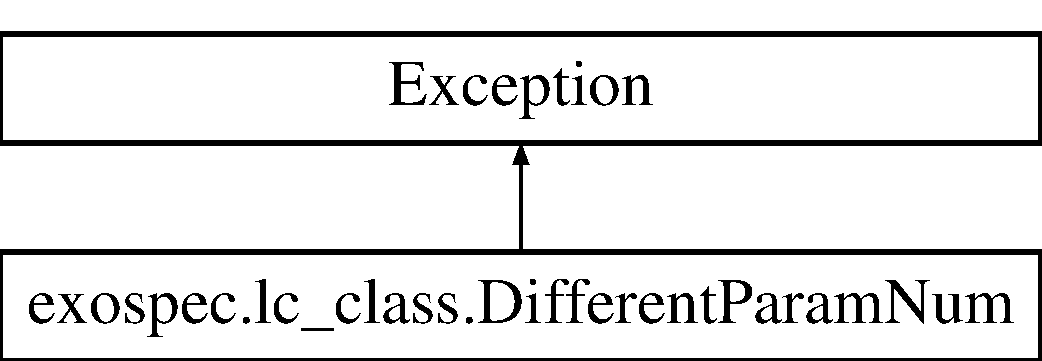
\includegraphics[height=2.000000cm]{classexospec_1_1lc__class_1_1_different_param_num}
\end{center}
\end{figure}


The documentation for this class was generated from the following file\+:\begin{DoxyCompactItemize}
\item 
/\+Users/heatherp/\+Documents/\+Courses/\+Computational/\+Project/\+Exoplanet\+Spectra/exospec/lc\+\_\+class.\+py\end{DoxyCompactItemize}

\hypertarget{classexospec_1_1read__input_1_1_empty_file}{}\section{exospec.\+read\+\_\+input.\+Empty\+File Class Reference}
\label{classexospec_1_1read__input_1_1_empty_file}\index{exospec.\+read\+\_\+input.\+Empty\+File@{exospec.\+read\+\_\+input.\+Empty\+File}}


Raise exception when the input file is empty or only has comments.  


Inheritance diagram for exospec.\+read\+\_\+input.\+Empty\+File\+:\begin{figure}[H]
\begin{center}
\leavevmode
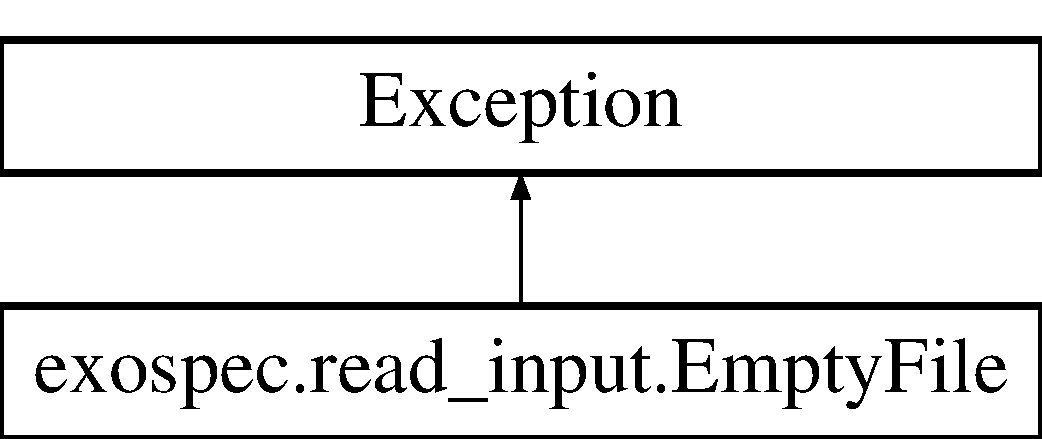
\includegraphics[height=2.000000cm]{classexospec_1_1read__input_1_1_empty_file}
\end{center}
\end{figure}


The documentation for this class was generated from the following file\+:\begin{DoxyCompactItemize}
\item 
/\+Users/heatherp/\+Documents/\+Courses/\+Computational/\+Project/\+Exoplanet\+Spectra/exospec/read\+\_\+input.\+py\end{DoxyCompactItemize}

\hypertarget{classexospec_1_1lc__class_1_1_empty_file}{}\section{exospec.\+lc\+\_\+class.\+Empty\+File Class Reference}
\label{classexospec_1_1lc__class_1_1_empty_file}\index{exospec.\+lc\+\_\+class.\+Empty\+File@{exospec.\+lc\+\_\+class.\+Empty\+File}}


Raise when the light curve file is empty.  


Inheritance diagram for exospec.\+lc\+\_\+class.\+Empty\+File\+:\begin{figure}[H]
\begin{center}
\leavevmode
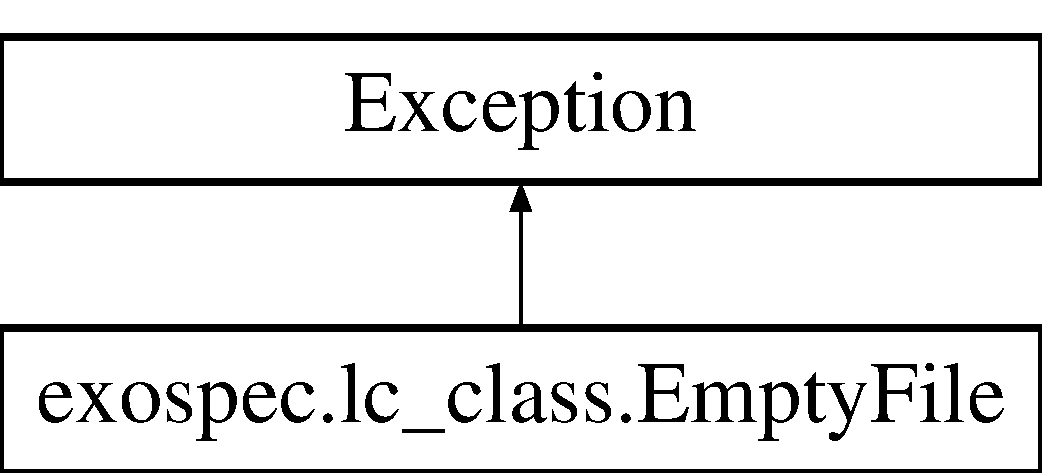
\includegraphics[height=2.000000cm]{classexospec_1_1lc__class_1_1_empty_file}
\end{center}
\end{figure}


The documentation for this class was generated from the following file\+:\begin{DoxyCompactItemize}
\item 
/\+Users/heatherp/\+Documents/\+Courses/\+Computational/\+Project/\+Exoplanet\+Spectra/exospec/lc\+\_\+class.\+py\end{DoxyCompactItemize}

\hypertarget{classexospec_1_1lc__class_1_1_empty_folder}{}\section{exospec.\+lc\+\_\+class.\+Empty\+Folder Class Reference}
\label{classexospec_1_1lc__class_1_1_empty_folder}\index{exospec.\+lc\+\_\+class.\+Empty\+Folder@{exospec.\+lc\+\_\+class.\+Empty\+Folder}}


Raise exception when the light curve folder is empty.  


Inheritance diagram for exospec.\+lc\+\_\+class.\+Empty\+Folder\+:\begin{figure}[H]
\begin{center}
\leavevmode
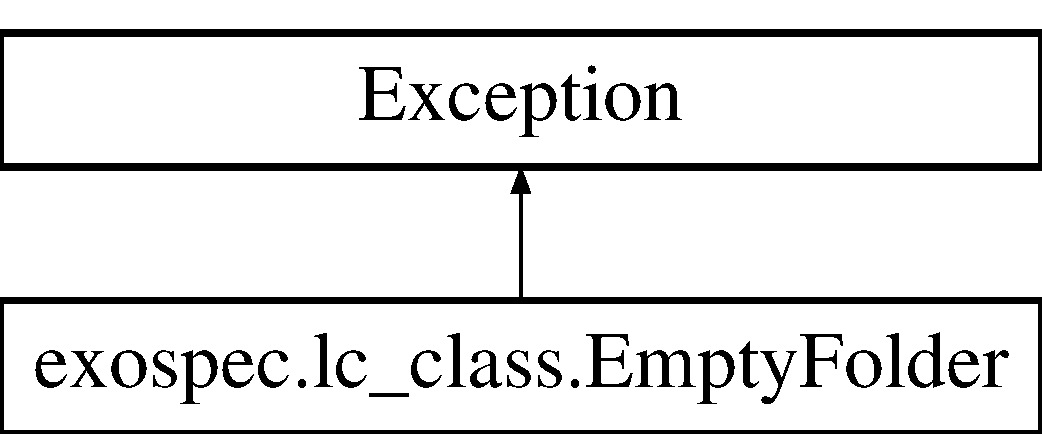
\includegraphics[height=2.000000cm]{classexospec_1_1lc__class_1_1_empty_folder}
\end{center}
\end{figure}


The documentation for this class was generated from the following file\+:\begin{DoxyCompactItemize}
\item 
lc\+\_\+class.\+py\end{DoxyCompactItemize}

\hypertarget{classexospec_1_1lc__class_1_1_incorrect_name_format}{}\section{exospec.\+lc\+\_\+class.\+Incorrect\+Name\+Format Class Reference}
\label{classexospec_1_1lc__class_1_1_incorrect_name_format}\index{exospec.\+lc\+\_\+class.\+Incorrect\+Name\+Format@{exospec.\+lc\+\_\+class.\+Incorrect\+Name\+Format}}


Raise when the light curve file name is not under the expected format sample\+\_\+lc\+\_\+$<$wavelength$>$.\+txt.  


Inheritance diagram for exospec.\+lc\+\_\+class.\+Incorrect\+Name\+Format\+:\begin{figure}[H]
\begin{center}
\leavevmode
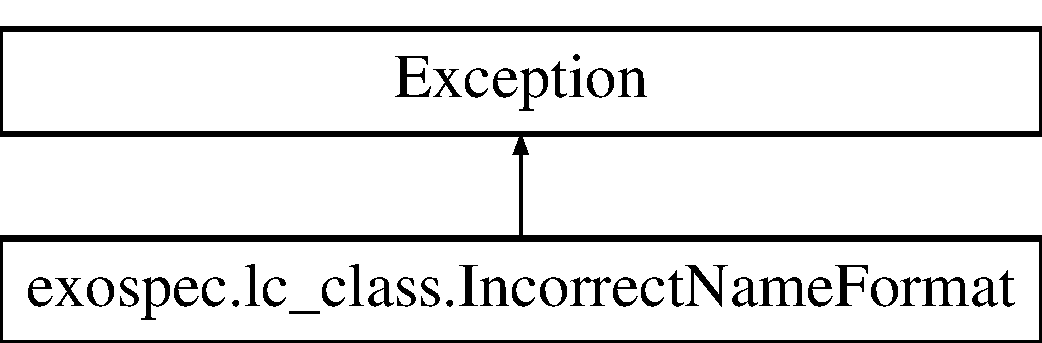
\includegraphics[height=2.000000cm]{classexospec_1_1lc__class_1_1_incorrect_name_format}
\end{center}
\end{figure}


The documentation for this class was generated from the following file\+:\begin{DoxyCompactItemize}
\item 
/\+Users/heatherp/\+Documents/\+Courses/\+Computational/\+Project/\+Exoplanet\+Spectra/exospec/lc\+\_\+class.\+py\end{DoxyCompactItemize}

\hypertarget{classexospec_1_1lc__class_1_1_light_curve}{}\section{exospec.\+lc\+\_\+class.\+Light\+Curve Class Reference}
\label{classexospec_1_1lc__class_1_1_light_curve}\index{exospec.\+lc\+\_\+class.\+Light\+Curve@{exospec.\+lc\+\_\+class.\+Light\+Curve}}


List all the light curve files in the indicated folder if the user decided to use another wavelength resolution than the one provided with the files, the code compute the resulting number of new wavelength to be used loop over the light curve files to get their file names and original wavelengths if the user decided to use a new wavelength resolution, the code computes the new wavelength to be used instantiate the new lc objects (with new wave\+\_\+bin\+\_\+size) Warning\+: The code is not able yet to handle situation where files\+\_\+num is not proportional to wave\+\_\+bin\+\_\+size.  


\subsection*{Public Member Functions}
\begin{DoxyCompactItemize}
\item 
\mbox{\Hypertarget{classexospec_1_1lc__class_1_1_light_curve_a231f0966a5321231cc9017956d7e037c}\label{classexospec_1_1lc__class_1_1_light_curve_a231f0966a5321231cc9017956d7e037c}} 
def {\bfseries \+\_\+\+\_\+init\+\_\+\+\_\+} (self, Path\+To\+LC, wave\+\_\+bin\+\_\+size)
\item 
def \hyperlink{classexospec_1_1lc__class_1_1_light_curve_aa0feb2d525e844a5f010939b3a8e9ae9}{L\+C\+\_\+dic} (self)
\begin{DoxyCompactList}\small\item\em Return L\+C\+\_\+dic. \end{DoxyCompactList}\item 
def \hyperlink{classexospec_1_1lc__class_1_1_light_curve_a9da0e4bf8f9ea153afb534d63fb7d24a}{wave\+\_\+length} (self)
\begin{DoxyCompactList}\small\item\em Return wave\+\_\+length. \end{DoxyCompactList}\item 
def \hyperlink{classexospec_1_1lc__class_1_1_light_curve_a8af62f3180b7d965c9d02ad92b1f0089}{new\+\_\+wave\+\_\+length} (self)
\begin{DoxyCompactList}\small\item\em Return new\+\_\+wave\+\_\+length. \end{DoxyCompactList}\item 
def \hyperlink{classexospec_1_1lc__class_1_1_light_curve_aa71fe5f0926727ae236782c414a08a4b}{store\+\_\+transit\+\_\+model} (self, transit\+\_\+model)
\begin{DoxyCompactList}\small\item\em Stores transit\+\_\+model. \end{DoxyCompactList}\end{DoxyCompactItemize}
\subsection*{Public Attributes}
\begin{DoxyCompactItemize}
\item 
\mbox{\Hypertarget{classexospec_1_1lc__class_1_1_light_curve_aad67f4c50ac516b103faff7218d395b4}\label{classexospec_1_1lc__class_1_1_light_curve_aad67f4c50ac516b103faff7218d395b4}} 
{\bfseries files\+\_\+list}
\item 
\mbox{\Hypertarget{classexospec_1_1lc__class_1_1_light_curve_a94e87b80871595e9ee15d29ef8bc1c15}\label{classexospec_1_1lc__class_1_1_light_curve_a94e87b80871595e9ee15d29ef8bc1c15}} 
{\bfseries files\+\_\+num}
\item 
\mbox{\Hypertarget{classexospec_1_1lc__class_1_1_light_curve_a818e9f5b159a68a971d7a7aaaac3cfb2}\label{classexospec_1_1lc__class_1_1_light_curve_a818e9f5b159a68a971d7a7aaaac3cfb2}} 
{\bfseries wave\+\_\+length}
\item 
\mbox{\Hypertarget{classexospec_1_1lc__class_1_1_light_curve_a86b7eae27d3c15065a096e1eb25a48f0}\label{classexospec_1_1lc__class_1_1_light_curve_a86b7eae27d3c15065a096e1eb25a48f0}} 
{\bfseries new\+\_\+wave\+\_\+length}
\item 
\mbox{\Hypertarget{classexospec_1_1lc__class_1_1_light_curve_a2bc92de5f90658957da35f6bf3050b7a}\label{classexospec_1_1lc__class_1_1_light_curve_a2bc92de5f90658957da35f6bf3050b7a}} 
{\bfseries L\+C\+\_\+dic}
\item 
\mbox{\Hypertarget{classexospec_1_1lc__class_1_1_light_curve_a02d9a3945664f48a03963beae70fc7b8}\label{classexospec_1_1lc__class_1_1_light_curve_a02d9a3945664f48a03963beae70fc7b8}} 
{\bfseries obj\+\_\+mcmc}
\item 
\mbox{\Hypertarget{classexospec_1_1lc__class_1_1_light_curve_a22f6adbcc1c7e2cd6833846908eb1b9c}\label{classexospec_1_1lc__class_1_1_light_curve_a22f6adbcc1c7e2cd6833846908eb1b9c}} 
{\bfseries obj\+\_\+chain}
\item 
\mbox{\Hypertarget{classexospec_1_1lc__class_1_1_light_curve_adf7758c000691cd491b4b428ad627fa1}\label{classexospec_1_1lc__class_1_1_light_curve_adf7758c000691cd491b4b428ad627fa1}} 
{\bfseries obj\+\_\+mcmc\+GP}
\item 
\mbox{\Hypertarget{classexospec_1_1lc__class_1_1_light_curve_ac00c2dab94929ffbf53f3de9c66e1d8a}\label{classexospec_1_1lc__class_1_1_light_curve_ac00c2dab94929ffbf53f3de9c66e1d8a}} 
{\bfseries obj\+\_\+chain\+GP}
\item 
\mbox{\Hypertarget{classexospec_1_1lc__class_1_1_light_curve_a02b2f724874285b53d4e788cb9b4e05d}\label{classexospec_1_1lc__class_1_1_light_curve_a02b2f724874285b53d4e788cb9b4e05d}} 
{\bfseries transit\+\_\+model}
\end{DoxyCompactItemize}


\subsection{Detailed Description}
List all the light curve files in the indicated folder if the user decided to use another wavelength resolution than the one provided with the files, the code compute the resulting number of new wavelength to be used loop over the light curve files to get their file names and original wavelengths if the user decided to use a new wavelength resolution, the code computes the new wavelength to be used instantiate the new lc objects (with new wave\+\_\+bin\+\_\+size) Warning\+: The code is not able yet to handle situation where files\+\_\+num is not proportional to wave\+\_\+bin\+\_\+size. 

\subsection{Member Function Documentation}
\mbox{\Hypertarget{classexospec_1_1lc__class_1_1_light_curve_aa0feb2d525e844a5f010939b3a8e9ae9}\label{classexospec_1_1lc__class_1_1_light_curve_aa0feb2d525e844a5f010939b3a8e9ae9}} 
\index{exospec\+::lc\+\_\+class\+::\+Light\+Curve@{exospec\+::lc\+\_\+class\+::\+Light\+Curve}!L\+C\+\_\+dic@{L\+C\+\_\+dic}}
\index{L\+C\+\_\+dic@{L\+C\+\_\+dic}!exospec\+::lc\+\_\+class\+::\+Light\+Curve@{exospec\+::lc\+\_\+class\+::\+Light\+Curve}}
\subsubsection{\texorpdfstring{L\+C\+\_\+dic()}{LC\_dic()}}
{\footnotesize\ttfamily def exospec.\+lc\+\_\+class.\+Light\+Curve.\+L\+C\+\_\+dic (\begin{DoxyParamCaption}\item[{}]{self }\end{DoxyParamCaption})}



Return L\+C\+\_\+dic. 

\begin{DoxyReturn}{Returns}
L\+C\+\_\+dic the dictionary that contains the light curve objects and which are references by their wavelength as keys 
\end{DoxyReturn}
\mbox{\Hypertarget{classexospec_1_1lc__class_1_1_light_curve_a8af62f3180b7d965c9d02ad92b1f0089}\label{classexospec_1_1lc__class_1_1_light_curve_a8af62f3180b7d965c9d02ad92b1f0089}} 
\index{exospec\+::lc\+\_\+class\+::\+Light\+Curve@{exospec\+::lc\+\_\+class\+::\+Light\+Curve}!new\+\_\+wave\+\_\+length@{new\+\_\+wave\+\_\+length}}
\index{new\+\_\+wave\+\_\+length@{new\+\_\+wave\+\_\+length}!exospec\+::lc\+\_\+class\+::\+Light\+Curve@{exospec\+::lc\+\_\+class\+::\+Light\+Curve}}
\subsubsection{\texorpdfstring{new\+\_\+wave\+\_\+length()}{new\_wave\_length()}}
{\footnotesize\ttfamily def exospec.\+lc\+\_\+class.\+Light\+Curve.\+new\+\_\+wave\+\_\+length (\begin{DoxyParamCaption}\item[{}]{self }\end{DoxyParamCaption})}



Return new\+\_\+wave\+\_\+length. 

\begin{DoxyReturn}{Returns}
new\+\_\+wave\+\_\+length a list containing the new user defined wavelength of the ligth curve objects 
\end{DoxyReturn}
\mbox{\Hypertarget{classexospec_1_1lc__class_1_1_light_curve_aa71fe5f0926727ae236782c414a08a4b}\label{classexospec_1_1lc__class_1_1_light_curve_aa71fe5f0926727ae236782c414a08a4b}} 
\index{exospec\+::lc\+\_\+class\+::\+Light\+Curve@{exospec\+::lc\+\_\+class\+::\+Light\+Curve}!store\+\_\+transit\+\_\+model@{store\+\_\+transit\+\_\+model}}
\index{store\+\_\+transit\+\_\+model@{store\+\_\+transit\+\_\+model}!exospec\+::lc\+\_\+class\+::\+Light\+Curve@{exospec\+::lc\+\_\+class\+::\+Light\+Curve}}
\subsubsection{\texorpdfstring{store\+\_\+transit\+\_\+model()}{store\_transit\_model()}}
{\footnotesize\ttfamily def exospec.\+lc\+\_\+class.\+Light\+Curve.\+store\+\_\+transit\+\_\+model (\begin{DoxyParamCaption}\item[{}]{self,  }\item[{}]{transit\+\_\+model }\end{DoxyParamCaption})}



Stores transit\+\_\+model. 


\begin{DoxyParams}{Parameters}
{\em transit\+\_\+model} & \\
\hline
\end{DoxyParams}
\mbox{\Hypertarget{classexospec_1_1lc__class_1_1_light_curve_a9da0e4bf8f9ea153afb534d63fb7d24a}\label{classexospec_1_1lc__class_1_1_light_curve_a9da0e4bf8f9ea153afb534d63fb7d24a}} 
\index{exospec\+::lc\+\_\+class\+::\+Light\+Curve@{exospec\+::lc\+\_\+class\+::\+Light\+Curve}!wave\+\_\+length@{wave\+\_\+length}}
\index{wave\+\_\+length@{wave\+\_\+length}!exospec\+::lc\+\_\+class\+::\+Light\+Curve@{exospec\+::lc\+\_\+class\+::\+Light\+Curve}}
\subsubsection{\texorpdfstring{wave\+\_\+length()}{wave\_length()}}
{\footnotesize\ttfamily def exospec.\+lc\+\_\+class.\+Light\+Curve.\+wave\+\_\+length (\begin{DoxyParamCaption}\item[{}]{self }\end{DoxyParamCaption})}



Return wave\+\_\+length. 

\begin{DoxyReturn}{Returns}
wave\+\_\+length a list containing the original wavelength of the ligth curve files 
\end{DoxyReturn}


The documentation for this class was generated from the following file\+:\begin{DoxyCompactItemize}
\item 
/\+Users/heatherp/\+Documents/\+Courses/\+Computational/\+Project/\+Exoplanet\+Spectra/exospec/lc\+\_\+class.\+py\end{DoxyCompactItemize}

\hypertarget{classexospec_1_1lc__class_1_1_light_curve_data}{}\section{exospec.\+lc\+\_\+class.\+Light\+Curve\+Data Class Reference}
\label{classexospec_1_1lc__class_1_1_light_curve_data}\index{exospec.\+lc\+\_\+class.\+Light\+Curve\+Data@{exospec.\+lc\+\_\+class.\+Light\+Curve\+Data}}


this class is used by the class \hyperlink{classexospec_1_1lc__class_1_1_light_curve}{Light\+Curve} to extract, store and process the data from the light curve files  


\subsection*{Public Member Functions}
\begin{DoxyCompactItemize}
\item 
\mbox{\Hypertarget{classexospec_1_1lc__class_1_1_light_curve_data_ae1113e4e3550f87c8d4339af1c8d1b6e}\label{classexospec_1_1lc__class_1_1_light_curve_data_ae1113e4e3550f87c8d4339af1c8d1b6e}} 
def {\bfseries \+\_\+\+\_\+init\+\_\+\+\_\+} (self, Path\+\_\+to\+\_\+files)
\item 
def \hyperlink{classexospec_1_1lc__class_1_1_light_curve_data_a33061fe920777987d5cc9936bd112d9e}{len\+\_\+file} (self)
\begin{DoxyCompactList}\small\item\em Returns len\+\_\+file. \end{DoxyCompactList}\item 
def \hyperlink{classexospec_1_1lc__class_1_1_light_curve_data_ad216feba69b805a0732a43555354c76d}{time} (self)
\begin{DoxyCompactList}\small\item\em Return time. \end{DoxyCompactList}\item 
def \hyperlink{classexospec_1_1lc__class_1_1_light_curve_data_a99a2aa168565aa5e6a0b2ec95aa92cff}{flux} (self)
\begin{DoxyCompactList}\small\item\em Returns flux. \end{DoxyCompactList}\item 
def \hyperlink{classexospec_1_1lc__class_1_1_light_curve_data_a4d3d200dc5af76cdd33f610c12ebba83}{ferr} (self)
\begin{DoxyCompactList}\small\item\em Returns ferr. \end{DoxyCompactList}\item 
def \hyperlink{classexospec_1_1lc__class_1_1_light_curve_data_a352d1d2bd0496d7117546a29b2c7cb34}{param\+\_\+num} (self)
\begin{DoxyCompactList}\small\item\em Returns param\+\_\+num. \end{DoxyCompactList}\item 
def \hyperlink{classexospec_1_1lc__class_1_1_light_curve_data_a515e685cc89aae396dc37212cff2e94b}{param\+\_\+name} (self)
\begin{DoxyCompactList}\small\item\em Returns param\+\_\+name. \end{DoxyCompactList}\item 
def \hyperlink{classexospec_1_1lc__class_1_1_light_curve_data_ab383d2dc1788a08a0336cb694f01c906}{param\+\_\+list} (self)
\begin{DoxyCompactList}\small\item\em Returns param\+\_\+list. \end{DoxyCompactList}\item 
def \hyperlink{classexospec_1_1lc__class_1_1_light_curve_data_ad09684789cb0431662a673f72aef7ac8}{new\+\_\+time\+\_\+bin} (self, bin\+\_\+size)
\begin{DoxyCompactList}\small\item\em Change the time resolution of a light curve object enables the user to use a new time resolution. \end{DoxyCompactList}\item 
def \hyperlink{classexospec_1_1lc__class_1_1_light_curve_data_a3e63540e9bb38ce3415d27527e8c6ba9}{plot\+\_\+flux\+\_\+time} (self, bin\+\_\+size)
\begin{DoxyCompactList}\small\item\em Plot the flux against the time plot the flux with a new time resolution using function new\+\_\+time\+\_\+bin. \end{DoxyCompactList}\item 
def \hyperlink{classexospec_1_1lc__class_1_1_light_curve_data_a917ef7c0956874d2c9c1696c02305ef5}{plot\+\_\+flux\+\_\+param} (self, param\+\_\+index)
\begin{DoxyCompactList}\small\item\em Plot the flux against a parameter plot the flux againt the parameter indicated by the user. \end{DoxyCompactList}\end{DoxyCompactItemize}
\subsection*{Public Attributes}
\begin{DoxyCompactItemize}
\item 
\mbox{\Hypertarget{classexospec_1_1lc__class_1_1_light_curve_data_adec28cf813c15d7c75f402d7bb51804d}\label{classexospec_1_1lc__class_1_1_light_curve_data_adec28cf813c15d7c75f402d7bb51804d}} 
{\bfseries len\+\_\+file}
\item 
\mbox{\Hypertarget{classexospec_1_1lc__class_1_1_light_curve_data_a118772717cee974c8f56534c1c4fa9bd}\label{classexospec_1_1lc__class_1_1_light_curve_data_a118772717cee974c8f56534c1c4fa9bd}} 
{\bfseries time}
\item 
\mbox{\Hypertarget{classexospec_1_1lc__class_1_1_light_curve_data_a8f871e916a7b560139181bf8cb9d0784}\label{classexospec_1_1lc__class_1_1_light_curve_data_a8f871e916a7b560139181bf8cb9d0784}} 
{\bfseries flux}
\item 
\mbox{\Hypertarget{classexospec_1_1lc__class_1_1_light_curve_data_adcc1b218150a87e12fd77a65103f4322}\label{classexospec_1_1lc__class_1_1_light_curve_data_adcc1b218150a87e12fd77a65103f4322}} 
{\bfseries ferr}
\item 
\mbox{\Hypertarget{classexospec_1_1lc__class_1_1_light_curve_data_a0e0ef1bb47bea5bf61b47493a49eb2c1}\label{classexospec_1_1lc__class_1_1_light_curve_data_a0e0ef1bb47bea5bf61b47493a49eb2c1}} 
{\bfseries param\+\_\+num}
\item 
\mbox{\Hypertarget{classexospec_1_1lc__class_1_1_light_curve_data_a2b6db36191285094a8456aba0f339b4a}\label{classexospec_1_1lc__class_1_1_light_curve_data_a2b6db36191285094a8456aba0f339b4a}} 
{\bfseries param\+\_\+name}
\item 
\mbox{\Hypertarget{classexospec_1_1lc__class_1_1_light_curve_data_a0d1f6258313a1e9ceb9bbe8ddf59eb76}\label{classexospec_1_1lc__class_1_1_light_curve_data_a0d1f6258313a1e9ceb9bbe8ddf59eb76}} 
{\bfseries param\+\_\+list}
\end{DoxyCompactItemize}


\subsection{Detailed Description}

\begin{DoxyParams}{Parameters}
{\em Path\+\_\+to\+\_\+files} & A list that contains the path(s) to the file(s) that will be used to create a light curve object (multiple files can be lumped together to create a ligh curve object) \\
\hline
\end{DoxyParams}


\subsection{Member Function Documentation}
\mbox{\Hypertarget{classexospec_1_1lc__class_1_1_light_curve_data_a4d3d200dc5af76cdd33f610c12ebba83}\label{classexospec_1_1lc__class_1_1_light_curve_data_a4d3d200dc5af76cdd33f610c12ebba83}} 
\index{exospec\+::lc\+\_\+class\+::\+Light\+Curve\+Data@{exospec\+::lc\+\_\+class\+::\+Light\+Curve\+Data}!ferr@{ferr}}
\index{ferr@{ferr}!exospec\+::lc\+\_\+class\+::\+Light\+Curve\+Data@{exospec\+::lc\+\_\+class\+::\+Light\+Curve\+Data}}
\subsubsection{\texorpdfstring{ferr()}{ferr()}}
{\footnotesize\ttfamily def exospec.\+lc\+\_\+class.\+Light\+Curve\+Data.\+ferr (\begin{DoxyParamCaption}\item[{}]{self }\end{DoxyParamCaption})}

\begin{DoxyReturn}{Returns}
ferr the error on the flux 
\end{DoxyReturn}
\mbox{\Hypertarget{classexospec_1_1lc__class_1_1_light_curve_data_a99a2aa168565aa5e6a0b2ec95aa92cff}\label{classexospec_1_1lc__class_1_1_light_curve_data_a99a2aa168565aa5e6a0b2ec95aa92cff}} 
\index{exospec\+::lc\+\_\+class\+::\+Light\+Curve\+Data@{exospec\+::lc\+\_\+class\+::\+Light\+Curve\+Data}!flux@{flux}}
\index{flux@{flux}!exospec\+::lc\+\_\+class\+::\+Light\+Curve\+Data@{exospec\+::lc\+\_\+class\+::\+Light\+Curve\+Data}}
\subsubsection{\texorpdfstring{flux()}{flux()}}
{\footnotesize\ttfamily def exospec.\+lc\+\_\+class.\+Light\+Curve\+Data.\+flux (\begin{DoxyParamCaption}\item[{}]{self }\end{DoxyParamCaption})}

\begin{DoxyReturn}{Returns}
flux the flux vector 
\end{DoxyReturn}
\mbox{\Hypertarget{classexospec_1_1lc__class_1_1_light_curve_data_a33061fe920777987d5cc9936bd112d9e}\label{classexospec_1_1lc__class_1_1_light_curve_data_a33061fe920777987d5cc9936bd112d9e}} 
\index{exospec\+::lc\+\_\+class\+::\+Light\+Curve\+Data@{exospec\+::lc\+\_\+class\+::\+Light\+Curve\+Data}!len\+\_\+file@{len\+\_\+file}}
\index{len\+\_\+file@{len\+\_\+file}!exospec\+::lc\+\_\+class\+::\+Light\+Curve\+Data@{exospec\+::lc\+\_\+class\+::\+Light\+Curve\+Data}}
\subsubsection{\texorpdfstring{len\+\_\+file()}{len\_file()}}
{\footnotesize\ttfamily def exospec.\+lc\+\_\+class.\+Light\+Curve\+Data.\+len\+\_\+file (\begin{DoxyParamCaption}\item[{}]{self }\end{DoxyParamCaption})}

\begin{DoxyReturn}{Returns}
len\+\_\+file the length of the light curve file 
\end{DoxyReturn}
\mbox{\Hypertarget{classexospec_1_1lc__class_1_1_light_curve_data_ad09684789cb0431662a673f72aef7ac8}\label{classexospec_1_1lc__class_1_1_light_curve_data_ad09684789cb0431662a673f72aef7ac8}} 
\index{exospec\+::lc\+\_\+class\+::\+Light\+Curve\+Data@{exospec\+::lc\+\_\+class\+::\+Light\+Curve\+Data}!new\+\_\+time\+\_\+bin@{new\+\_\+time\+\_\+bin}}
\index{new\+\_\+time\+\_\+bin@{new\+\_\+time\+\_\+bin}!exospec\+::lc\+\_\+class\+::\+Light\+Curve\+Data@{exospec\+::lc\+\_\+class\+::\+Light\+Curve\+Data}}
\subsubsection{\texorpdfstring{new\+\_\+time\+\_\+bin()}{new\_time\_bin()}}
{\footnotesize\ttfamily def exospec.\+lc\+\_\+class.\+Light\+Curve\+Data.\+new\+\_\+time\+\_\+bin (\begin{DoxyParamCaption}\item[{}]{self,  }\item[{}]{bin\+\_\+size }\end{DoxyParamCaption})}


\begin{DoxyParams}{Parameters}
{\em bin\+\_\+size} & number of time points to lump together \\
\hline
\end{DoxyParams}
\mbox{\Hypertarget{classexospec_1_1lc__class_1_1_light_curve_data_ab383d2dc1788a08a0336cb694f01c906}\label{classexospec_1_1lc__class_1_1_light_curve_data_ab383d2dc1788a08a0336cb694f01c906}} 
\index{exospec\+::lc\+\_\+class\+::\+Light\+Curve\+Data@{exospec\+::lc\+\_\+class\+::\+Light\+Curve\+Data}!param\+\_\+list@{param\+\_\+list}}
\index{param\+\_\+list@{param\+\_\+list}!exospec\+::lc\+\_\+class\+::\+Light\+Curve\+Data@{exospec\+::lc\+\_\+class\+::\+Light\+Curve\+Data}}
\subsubsection{\texorpdfstring{param\+\_\+list()}{param\_list()}}
{\footnotesize\ttfamily def exospec.\+lc\+\_\+class.\+Light\+Curve\+Data.\+param\+\_\+list (\begin{DoxyParamCaption}\item[{}]{self }\end{DoxyParamCaption})}

\begin{DoxyReturn}{Returns}
param\+\_\+list a list containing the parameters 
\end{DoxyReturn}
\mbox{\Hypertarget{classexospec_1_1lc__class_1_1_light_curve_data_a515e685cc89aae396dc37212cff2e94b}\label{classexospec_1_1lc__class_1_1_light_curve_data_a515e685cc89aae396dc37212cff2e94b}} 
\index{exospec\+::lc\+\_\+class\+::\+Light\+Curve\+Data@{exospec\+::lc\+\_\+class\+::\+Light\+Curve\+Data}!param\+\_\+name@{param\+\_\+name}}
\index{param\+\_\+name@{param\+\_\+name}!exospec\+::lc\+\_\+class\+::\+Light\+Curve\+Data@{exospec\+::lc\+\_\+class\+::\+Light\+Curve\+Data}}
\subsubsection{\texorpdfstring{param\+\_\+name()}{param\_name()}}
{\footnotesize\ttfamily def exospec.\+lc\+\_\+class.\+Light\+Curve\+Data.\+param\+\_\+name (\begin{DoxyParamCaption}\item[{}]{self }\end{DoxyParamCaption})}

\begin{DoxyReturn}{Returns}
param\+\_\+name a list containing the names of the parameters 
\end{DoxyReturn}
\mbox{\Hypertarget{classexospec_1_1lc__class_1_1_light_curve_data_a352d1d2bd0496d7117546a29b2c7cb34}\label{classexospec_1_1lc__class_1_1_light_curve_data_a352d1d2bd0496d7117546a29b2c7cb34}} 
\index{exospec\+::lc\+\_\+class\+::\+Light\+Curve\+Data@{exospec\+::lc\+\_\+class\+::\+Light\+Curve\+Data}!param\+\_\+num@{param\+\_\+num}}
\index{param\+\_\+num@{param\+\_\+num}!exospec\+::lc\+\_\+class\+::\+Light\+Curve\+Data@{exospec\+::lc\+\_\+class\+::\+Light\+Curve\+Data}}
\subsubsection{\texorpdfstring{param\+\_\+num()}{param\_num()}}
{\footnotesize\ttfamily def exospec.\+lc\+\_\+class.\+Light\+Curve\+Data.\+param\+\_\+num (\begin{DoxyParamCaption}\item[{}]{self }\end{DoxyParamCaption})}

\begin{DoxyReturn}{Returns}
param\+\_\+num the number of parameters defined in the light curve file 
\end{DoxyReturn}
\mbox{\Hypertarget{classexospec_1_1lc__class_1_1_light_curve_data_a917ef7c0956874d2c9c1696c02305ef5}\label{classexospec_1_1lc__class_1_1_light_curve_data_a917ef7c0956874d2c9c1696c02305ef5}} 
\index{exospec\+::lc\+\_\+class\+::\+Light\+Curve\+Data@{exospec\+::lc\+\_\+class\+::\+Light\+Curve\+Data}!plot\+\_\+flux\+\_\+param@{plot\+\_\+flux\+\_\+param}}
\index{plot\+\_\+flux\+\_\+param@{plot\+\_\+flux\+\_\+param}!exospec\+::lc\+\_\+class\+::\+Light\+Curve\+Data@{exospec\+::lc\+\_\+class\+::\+Light\+Curve\+Data}}
\subsubsection{\texorpdfstring{plot\+\_\+flux\+\_\+param()}{plot\_flux\_param()}}
{\footnotesize\ttfamily def exospec.\+lc\+\_\+class.\+Light\+Curve\+Data.\+plot\+\_\+flux\+\_\+param (\begin{DoxyParamCaption}\item[{}]{self,  }\item[{}]{param\+\_\+index }\end{DoxyParamCaption})}


\begin{DoxyParams}{Parameters}
{\em param\+\_\+index} & the index of the param selected by the user in param\+\_\+list \\
\hline
\end{DoxyParams}
\mbox{\Hypertarget{classexospec_1_1lc__class_1_1_light_curve_data_a3e63540e9bb38ce3415d27527e8c6ba9}\label{classexospec_1_1lc__class_1_1_light_curve_data_a3e63540e9bb38ce3415d27527e8c6ba9}} 
\index{exospec\+::lc\+\_\+class\+::\+Light\+Curve\+Data@{exospec\+::lc\+\_\+class\+::\+Light\+Curve\+Data}!plot\+\_\+flux\+\_\+time@{plot\+\_\+flux\+\_\+time}}
\index{plot\+\_\+flux\+\_\+time@{plot\+\_\+flux\+\_\+time}!exospec\+::lc\+\_\+class\+::\+Light\+Curve\+Data@{exospec\+::lc\+\_\+class\+::\+Light\+Curve\+Data}}
\subsubsection{\texorpdfstring{plot\+\_\+flux\+\_\+time()}{plot\_flux\_time()}}
{\footnotesize\ttfamily def exospec.\+lc\+\_\+class.\+Light\+Curve\+Data.\+plot\+\_\+flux\+\_\+time (\begin{DoxyParamCaption}\item[{}]{self,  }\item[{}]{bin\+\_\+size }\end{DoxyParamCaption})}


\begin{DoxyParams}{Parameters}
{\em bin\+\_\+size} & number of time points to lump together \\
\hline
\end{DoxyParams}
\mbox{\Hypertarget{classexospec_1_1lc__class_1_1_light_curve_data_ad216feba69b805a0732a43555354c76d}\label{classexospec_1_1lc__class_1_1_light_curve_data_ad216feba69b805a0732a43555354c76d}} 
\index{exospec\+::lc\+\_\+class\+::\+Light\+Curve\+Data@{exospec\+::lc\+\_\+class\+::\+Light\+Curve\+Data}!time@{time}}
\index{time@{time}!exospec\+::lc\+\_\+class\+::\+Light\+Curve\+Data@{exospec\+::lc\+\_\+class\+::\+Light\+Curve\+Data}}
\subsubsection{\texorpdfstring{time()}{time()}}
{\footnotesize\ttfamily def exospec.\+lc\+\_\+class.\+Light\+Curve\+Data.\+time (\begin{DoxyParamCaption}\item[{}]{self }\end{DoxyParamCaption})}

\begin{DoxyReturn}{Returns}
time the time vector 
\end{DoxyReturn}


The documentation for this class was generated from the following file\+:\begin{DoxyCompactItemize}
\item 
/\+Users/heatherp/\+Documents/\+Courses/\+Computational/\+Project/\+Exoplanet\+Spectra/exospec/lc\+\_\+class.\+py\end{DoxyCompactItemize}

\hypertarget{classexospec_1_1mcmc_1_1_m_c_m_c}{}\section{exospec.\+mcmc.\+M\+C\+MC Class Reference}
\label{classexospec_1_1mcmc_1_1_m_c_m_c}\index{exospec.\+mcmc.\+M\+C\+MC@{exospec.\+mcmc.\+M\+C\+MC}}


Class to run \hyperlink{classexospec_1_1mcmc_1_1_m_c_m_c}{M\+C\+MC} to fit curve and produce diagnostic plots and statistics Uses emcee (to run \hyperlink{classexospec_1_1mcmc_1_1_m_c_m_c}{M\+C\+MC}) and corner (to produce triangle plots)  


Inheritance diagram for exospec.\+mcmc.\+M\+C\+MC\+:\begin{figure}[H]
\begin{center}
\leavevmode
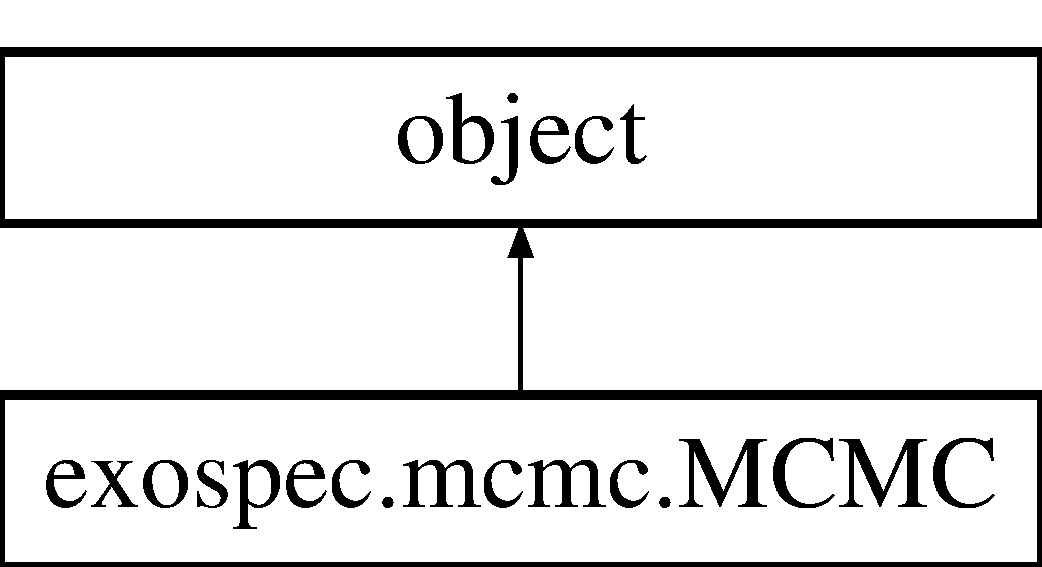
\includegraphics[height=2.000000cm]{classexospec_1_1mcmc_1_1_m_c_m_c}
\end{center}
\end{figure}
\subsection*{Public Member Functions}
\begin{DoxyCompactItemize}
\item 
def \hyperlink{classexospec_1_1mcmc_1_1_m_c_m_c_aae17f42d9fa567e61df69f7c808aa931}{\+\_\+\+\_\+init\+\_\+\+\_\+} (self, t, val, err, ln\+\_\+prob\+\_\+fn, transit\+\_\+params, hyper\+\_\+params, num\+\_\+walkers, num\+\_\+threads)
\begin{DoxyCompactList}\small\item\em The constructor. \end{DoxyCompactList}\item 
def \hyperlink{classexospec_1_1mcmc_1_1_m_c_m_c_af103863b006ff9225432bdc8b2e90d81}{run} (self, pos, burnin\+\_\+steps, production\+\_\+run\+\_\+steps)
\begin{DoxyCompactList}\small\item\em Runs the \hyperlink{classexospec_1_1mcmc_1_1_m_c_m_c}{M\+C\+MC} should run emcee given a log probability function result is the \hyperlink{classexospec_1_1mcmc_1_1_m_c_m_c}{M\+C\+MC} chains which are saved as an object attribute. \end{DoxyCompactList}\item 
def \hyperlink{classexospec_1_1mcmc_1_1_m_c_m_c_ad20ecaec3fc481c3ab87ad7c4c0439bc}{save\+\_\+chain} (self, filename)
\begin{DoxyCompactList}\small\item\em Saves the chain as a numpy array. \end{DoxyCompactList}\item 
def \hyperlink{classexospec_1_1mcmc_1_1_m_c_m_c_afec10cdfb36657e6e1c013bbd563bd71}{get\+\_\+mean\+\_\+acceptance\+\_\+fraction} (self)
\begin{DoxyCompactList}\small\item\em Allows the user to access the mean acceptance fraction The mean acceptance fractions should be between about 0.\+25 and 0.\+5. \end{DoxyCompactList}\item 
def \hyperlink{classexospec_1_1mcmc_1_1_m_c_m_c_a7fe8d9326590fe7cc875fa5118eaa617}{get\+\_\+median\+\_\+and\+\_\+errors} (self)
\begin{DoxyCompactList}\small\item\em Best fit parameters and 1 sigma errors. \end{DoxyCompactList}\item 
def \hyperlink{classexospec_1_1mcmc_1_1_m_c_m_c_af240e8deac4470da704239926ea56822}{triangle\+\_\+plot} (self, extra\+\_\+burnin\+\_\+steps=0, theta\+\_\+true=None, plot\+\_\+transit\+\_\+params=True, plot\+\_\+hyper\+\_\+params=True, save\+\_\+as\+\_\+dir=\char`\"{}.\char`\"{}, save\+\_\+as\+\_\+name=\char`\"{}triangle.\+png\char`\"{})
\begin{DoxyCompactList}\small\item\em Makes a triangle plot If an error is encountered the function returns 1 but does not raise an exception. \end{DoxyCompactList}\item 
def \hyperlink{classexospec_1_1mcmc_1_1_m_c_m_c_a741c2882baef53c1fa19b2c086ec8261}{walker\+\_\+plot} (self, extra\+\_\+burnin\+\_\+steps=0, theta\+\_\+true=None, plot\+\_\+transit\+\_\+params=True, plot\+\_\+hyper\+\_\+params=True, save\+\_\+as\+\_\+dir=\char`\"{}.\char`\"{}, save\+\_\+as\+\_\+name=\char`\"{}walkers.\+png\char`\"{})
\begin{DoxyCompactList}\small\item\em Plots the chains of each walker and a histogram showing how each parameter was sampled If an error is encountered the function returns 1 but does not raise an exception. \end{DoxyCompactList}\item 
def \hyperlink{classexospec_1_1mcmc_1_1_m_c_m_c_ab2c5cc870e2b384534404f3bc667e039}{light\+\_\+curve\+\_\+plot} (self, model, extra\+\_\+burnin\+\_\+steps=0, theta\+\_\+true=None, plot\+\_\+transit\+\_\+params=True, plot\+\_\+hyper\+\_\+params=True, save\+\_\+as\+\_\+dir=\char`\"{}.\char`\"{}, save\+\_\+as\+\_\+name=\char`\"{}light\+\_\+curve\char`\"{})
\begin{DoxyCompactList}\small\item\em Plots the chains of each walker and a histogram showing how each parameter was sampled If an error is encountered the function returns 1 but does not raise an exception. \end{DoxyCompactList}\end{DoxyCompactItemize}


\subsection{Constructor \& Destructor Documentation}
\mbox{\Hypertarget{classexospec_1_1mcmc_1_1_m_c_m_c_aae17f42d9fa567e61df69f7c808aa931}\label{classexospec_1_1mcmc_1_1_m_c_m_c_aae17f42d9fa567e61df69f7c808aa931}} 
\index{exospec\+::mcmc\+::\+M\+C\+MC@{exospec\+::mcmc\+::\+M\+C\+MC}!\+\_\+\+\_\+init\+\_\+\+\_\+@{\+\_\+\+\_\+init\+\_\+\+\_\+}}
\index{\+\_\+\+\_\+init\+\_\+\+\_\+@{\+\_\+\+\_\+init\+\_\+\+\_\+}!exospec\+::mcmc\+::\+M\+C\+MC@{exospec\+::mcmc\+::\+M\+C\+MC}}
\subsubsection{\texorpdfstring{\+\_\+\+\_\+init\+\_\+\+\_\+()}{\_\_init\_\_()}}
{\footnotesize\ttfamily def exospec.\+mcmc.\+M\+C\+M\+C.\+\_\+\+\_\+init\+\_\+\+\_\+ (\begin{DoxyParamCaption}\item[{}]{self,  }\item[{}]{t,  }\item[{}]{val,  }\item[{}]{err,  }\item[{}]{ln\+\_\+prob\+\_\+fn,  }\item[{}]{transit\+\_\+params,  }\item[{}]{hyper\+\_\+params,  }\item[{}]{num\+\_\+walkers,  }\item[{}]{num\+\_\+threads }\end{DoxyParamCaption})}


\begin{DoxyParams}{Parameters}
{\em self} & The object pointer \\
\hline
{\em t} & A numpy array of the independent variable for the data \\
\hline
{\em val} & A numpy array of the dependent variable for the data \\
\hline
{\em err} & A numpy array of the errors on the dependent variable \\
\hline
{\em ln\+\_\+prob\+\_\+fn} & The log probability function to be sampled \\
\hline
{\em transit\+\_\+params} & A list of the names of the curve\textquotesingle{}s parameters \\
\hline
{\em hyper\+\_\+params} & A list of the names of noise parameters \\
\hline
{\em num\+\_\+walkers} & Integer giving the number of walkers for the \hyperlink{classexospec_1_1mcmc_1_1_m_c_m_c}{M\+C\+MC} run \\
\hline
{\em num\+\_\+threads} & Integer giving the number of threads to use per core \\
\hline
\end{DoxyParams}


\subsection{Member Function Documentation}
\mbox{\Hypertarget{classexospec_1_1mcmc_1_1_m_c_m_c_afec10cdfb36657e6e1c013bbd563bd71}\label{classexospec_1_1mcmc_1_1_m_c_m_c_afec10cdfb36657e6e1c013bbd563bd71}} 
\index{exospec\+::mcmc\+::\+M\+C\+MC@{exospec\+::mcmc\+::\+M\+C\+MC}!get\+\_\+mean\+\_\+acceptance\+\_\+fraction@{get\+\_\+mean\+\_\+acceptance\+\_\+fraction}}
\index{get\+\_\+mean\+\_\+acceptance\+\_\+fraction@{get\+\_\+mean\+\_\+acceptance\+\_\+fraction}!exospec\+::mcmc\+::\+M\+C\+MC@{exospec\+::mcmc\+::\+M\+C\+MC}}
\subsubsection{\texorpdfstring{get\+\_\+mean\+\_\+acceptance\+\_\+fraction()}{get\_mean\_acceptance\_fraction()}}
{\footnotesize\ttfamily def exospec.\+mcmc.\+M\+C\+M\+C.\+get\+\_\+mean\+\_\+acceptance\+\_\+fraction (\begin{DoxyParamCaption}\item[{}]{self }\end{DoxyParamCaption})}


\begin{DoxyParams}{Parameters}
{\em self} & The object pointer \\
\hline
\end{DoxyParams}
\begin{DoxyReturn}{Returns}
Mean acceptance fraction 
\end{DoxyReturn}
\mbox{\Hypertarget{classexospec_1_1mcmc_1_1_m_c_m_c_a7fe8d9326590fe7cc875fa5118eaa617}\label{classexospec_1_1mcmc_1_1_m_c_m_c_a7fe8d9326590fe7cc875fa5118eaa617}} 
\index{exospec\+::mcmc\+::\+M\+C\+MC@{exospec\+::mcmc\+::\+M\+C\+MC}!get\+\_\+median\+\_\+and\+\_\+errors@{get\+\_\+median\+\_\+and\+\_\+errors}}
\index{get\+\_\+median\+\_\+and\+\_\+errors@{get\+\_\+median\+\_\+and\+\_\+errors}!exospec\+::mcmc\+::\+M\+C\+MC@{exospec\+::mcmc\+::\+M\+C\+MC}}
\subsubsection{\texorpdfstring{get\+\_\+median\+\_\+and\+\_\+errors()}{get\_median\_and\_errors()}}
{\footnotesize\ttfamily def exospec.\+mcmc.\+M\+C\+M\+C.\+get\+\_\+median\+\_\+and\+\_\+errors (\begin{DoxyParamCaption}\item[{}]{self }\end{DoxyParamCaption})}


\begin{DoxyParams}{Parameters}
{\em self} & The object pointer \\
\hline
\end{DoxyParams}
\begin{DoxyReturn}{Returns}
Three numpy arrays giving the median and one sigma errors for each parameter 
\end{DoxyReturn}
\mbox{\Hypertarget{classexospec_1_1mcmc_1_1_m_c_m_c_ab2c5cc870e2b384534404f3bc667e039}\label{classexospec_1_1mcmc_1_1_m_c_m_c_ab2c5cc870e2b384534404f3bc667e039}} 
\index{exospec\+::mcmc\+::\+M\+C\+MC@{exospec\+::mcmc\+::\+M\+C\+MC}!light\+\_\+curve\+\_\+plot@{light\+\_\+curve\+\_\+plot}}
\index{light\+\_\+curve\+\_\+plot@{light\+\_\+curve\+\_\+plot}!exospec\+::mcmc\+::\+M\+C\+MC@{exospec\+::mcmc\+::\+M\+C\+MC}}
\subsubsection{\texorpdfstring{light\+\_\+curve\+\_\+plot()}{light\_curve\_plot()}}
{\footnotesize\ttfamily def exospec.\+mcmc.\+M\+C\+M\+C.\+light\+\_\+curve\+\_\+plot (\begin{DoxyParamCaption}\item[{}]{self,  }\item[{}]{model,  }\item[{}]{extra\+\_\+burnin\+\_\+steps = {\ttfamily 0},  }\item[{}]{theta\+\_\+true = {\ttfamily None},  }\item[{}]{plot\+\_\+transit\+\_\+params = {\ttfamily True},  }\item[{}]{plot\+\_\+hyper\+\_\+params = {\ttfamily True},  }\item[{}]{save\+\_\+as\+\_\+dir = {\ttfamily \char`\"{}.\char`\"{}},  }\item[{}]{save\+\_\+as\+\_\+name = {\ttfamily \char`\"{}light\+\_\+curve\char`\"{}} }\end{DoxyParamCaption})}

These plots are useful for visualization but should not cause the code to crash, as the main purpose is to create and save the \hyperlink{classexospec_1_1mcmc_1_1_m_c_m_c}{M\+C\+MC} chains 
\begin{DoxyParams}{Parameters}
{\em self} & The object pointer \\
\hline
{\em model} & A function that returns the lightcurve shape as a function of the light curve parameters and time \\
\hline
{\em extra\+\_\+burnin\+\_\+steps} & Number of steps (in addition to burnin\+\_\+steps from run) at the start of each chain to neglect \\
\hline
{\em theta\+\_\+true} & Numpy array of true parameter values if known (used for test data) \\
\hline
{\em plot\+\_\+transit\+\_\+params} & Boolean value specifying whether or not to plot the transit parameters \\
\hline
{\em plot\+\_\+hyper\+\_\+params} & Boolean value specifying whether or not to plot the hyper parameters \\
\hline
{\em save\+\_\+as\+\_\+dir} & Directory where plot should be saved. Default is current working Directory \\
\hline
{\em save\+\_\+as\+\_\+name} & Name under which plot should be saved \\
\hline
\end{DoxyParams}

\begin{DoxyRetVals}{Return values}
{\em 0} & if successful \\
\hline
{\em 1} & on failure \\
\hline
\end{DoxyRetVals}
\mbox{\Hypertarget{classexospec_1_1mcmc_1_1_m_c_m_c_af103863b006ff9225432bdc8b2e90d81}\label{classexospec_1_1mcmc_1_1_m_c_m_c_af103863b006ff9225432bdc8b2e90d81}} 
\index{exospec\+::mcmc\+::\+M\+C\+MC@{exospec\+::mcmc\+::\+M\+C\+MC}!run@{run}}
\index{run@{run}!exospec\+::mcmc\+::\+M\+C\+MC@{exospec\+::mcmc\+::\+M\+C\+MC}}
\subsubsection{\texorpdfstring{run()}{run()}}
{\footnotesize\ttfamily def exospec.\+mcmc.\+M\+C\+M\+C.\+run (\begin{DoxyParamCaption}\item[{}]{self,  }\item[{}]{pos,  }\item[{}]{burnin\+\_\+steps,  }\item[{}]{production\+\_\+run\+\_\+steps }\end{DoxyParamCaption})}


\begin{DoxyParams}{Parameters}
{\em self} & The object pointer \\
\hline
{\em pos} & A 2D numpy array giving the initial positions of the walkers in parameter space \\
\hline
{\em burnin\+\_\+steps} & An integer giving the number of initial steps to take to start exploring the parameter space before starting to save the chains \\
\hline
{\em production\+\_\+run\+\_\+steps} & The number of steps to take for each walker after the burnin phase \\
\hline
\end{DoxyParams}
\begin{DoxyReturn}{Returns}
A 2D numpy array with all the samples for each of the transit and hyper parameters 
\end{DoxyReturn}
\mbox{\Hypertarget{classexospec_1_1mcmc_1_1_m_c_m_c_ad20ecaec3fc481c3ab87ad7c4c0439bc}\label{classexospec_1_1mcmc_1_1_m_c_m_c_ad20ecaec3fc481c3ab87ad7c4c0439bc}} 
\index{exospec\+::mcmc\+::\+M\+C\+MC@{exospec\+::mcmc\+::\+M\+C\+MC}!save\+\_\+chain@{save\+\_\+chain}}
\index{save\+\_\+chain@{save\+\_\+chain}!exospec\+::mcmc\+::\+M\+C\+MC@{exospec\+::mcmc\+::\+M\+C\+MC}}
\subsubsection{\texorpdfstring{save\+\_\+chain()}{save\_chain()}}
{\footnotesize\ttfamily def exospec.\+mcmc.\+M\+C\+M\+C.\+save\+\_\+chain (\begin{DoxyParamCaption}\item[{}]{self,  }\item[{}]{filename }\end{DoxyParamCaption})}


\begin{DoxyParams}{Parameters}
{\em self} & The object pointer \\
\hline
{\em filename} & The filename including path where the chains will be saved \\
\hline
\end{DoxyParams}

\begin{DoxyRetVals}{Return values}
{\em 0} & if successful \\
\hline
{\em 1} & if an IO error occurs or if the chain is empty \\
\hline
\end{DoxyRetVals}
\mbox{\Hypertarget{classexospec_1_1mcmc_1_1_m_c_m_c_af240e8deac4470da704239926ea56822}\label{classexospec_1_1mcmc_1_1_m_c_m_c_af240e8deac4470da704239926ea56822}} 
\index{exospec\+::mcmc\+::\+M\+C\+MC@{exospec\+::mcmc\+::\+M\+C\+MC}!triangle\+\_\+plot@{triangle\+\_\+plot}}
\index{triangle\+\_\+plot@{triangle\+\_\+plot}!exospec\+::mcmc\+::\+M\+C\+MC@{exospec\+::mcmc\+::\+M\+C\+MC}}
\subsubsection{\texorpdfstring{triangle\+\_\+plot()}{triangle\_plot()}}
{\footnotesize\ttfamily def exospec.\+mcmc.\+M\+C\+M\+C.\+triangle\+\_\+plot (\begin{DoxyParamCaption}\item[{}]{self,  }\item[{}]{extra\+\_\+burnin\+\_\+steps = {\ttfamily 0},  }\item[{}]{theta\+\_\+true = {\ttfamily None},  }\item[{}]{plot\+\_\+transit\+\_\+params = {\ttfamily True},  }\item[{}]{plot\+\_\+hyper\+\_\+params = {\ttfamily True},  }\item[{}]{save\+\_\+as\+\_\+dir = {\ttfamily \char`\"{}.\char`\"{}},  }\item[{}]{save\+\_\+as\+\_\+name = {\ttfamily \char`\"{}triangle.png\char`\"{}} }\end{DoxyParamCaption})}

These plots are useful for visualization but should not cause the code to crash, as the main purpose of the code is to create and save the \hyperlink{classexospec_1_1mcmc_1_1_m_c_m_c}{M\+C\+MC} chains. 
\begin{DoxyParams}{Parameters}
{\em self} & The object pointer \\
\hline
{\em extra\+\_\+burnin\+\_\+steps} & Number of steps (in addition to burnin\+\_\+steps from run) at the start of each chain to neglect \\
\hline
{\em theta\+\_\+true} & Numpy array of true parameter values for the parameters to be plotted (only used for test data) \\
\hline
{\em plot\+\_\+transit\+\_\+params} & Boolean value specifying whether or not to plot the transit parameters \\
\hline
{\em plot\+\_\+hyper\+\_\+params} & Boolean value specifying whether or not to plot the hyper parameters \\
\hline
{\em save\+\_\+as\+\_\+dir} & Directory where plot should be saved. Default is current working Directory \\
\hline
{\em save\+\_\+as\+\_\+name} & Name under which plot should be saved \\
\hline
\end{DoxyParams}

\begin{DoxyRetVals}{Return values}
{\em 0} & if successful \\
\hline
{\em 1} & on failure \\
\hline
\end{DoxyRetVals}
\mbox{\Hypertarget{classexospec_1_1mcmc_1_1_m_c_m_c_a741c2882baef53c1fa19b2c086ec8261}\label{classexospec_1_1mcmc_1_1_m_c_m_c_a741c2882baef53c1fa19b2c086ec8261}} 
\index{exospec\+::mcmc\+::\+M\+C\+MC@{exospec\+::mcmc\+::\+M\+C\+MC}!walker\+\_\+plot@{walker\+\_\+plot}}
\index{walker\+\_\+plot@{walker\+\_\+plot}!exospec\+::mcmc\+::\+M\+C\+MC@{exospec\+::mcmc\+::\+M\+C\+MC}}
\subsubsection{\texorpdfstring{walker\+\_\+plot()}{walker\_plot()}}
{\footnotesize\ttfamily def exospec.\+mcmc.\+M\+C\+M\+C.\+walker\+\_\+plot (\begin{DoxyParamCaption}\item[{}]{self,  }\item[{}]{extra\+\_\+burnin\+\_\+steps = {\ttfamily 0},  }\item[{}]{theta\+\_\+true = {\ttfamily None},  }\item[{}]{plot\+\_\+transit\+\_\+params = {\ttfamily True},  }\item[{}]{plot\+\_\+hyper\+\_\+params = {\ttfamily True},  }\item[{}]{save\+\_\+as\+\_\+dir = {\ttfamily \char`\"{}.\char`\"{}},  }\item[{}]{save\+\_\+as\+\_\+name = {\ttfamily \char`\"{}walkers.png\char`\"{}} }\end{DoxyParamCaption})}

These plots are useful for visualization but should not cause the code to crash, as the main purpose is to create and save the \hyperlink{classexospec_1_1mcmc_1_1_m_c_m_c}{M\+C\+MC} chains 
\begin{DoxyParams}{Parameters}
{\em self} & The object pointer \\
\hline
{\em extra\+\_\+burnin\+\_\+steps} & Number of steps (in addition to burnin\+\_\+steps from run) at the start of each chain to neglect \\
\hline
{\em theta\+\_\+true} & Numpy array of true parameter values if known (used for test data) \\
\hline
{\em plot\+\_\+transit\+\_\+params} & Boolean value specifying whether or not to plot the transit parameters \\
\hline
{\em plot\+\_\+hyper\+\_\+params} & Boolean value specifying whether or not to plot the hyper parameters \\
\hline
{\em save\+\_\+as\+\_\+dir} & Directory where plot should be saved. Default is current working Directory \\
\hline
{\em save\+\_\+as\+\_\+name} & Name under which plot should be saved \\
\hline
\end{DoxyParams}

\begin{DoxyRetVals}{Return values}
{\em 0} & if successful \\
\hline
{\em 1} & on failure \\
\hline
\end{DoxyRetVals}


The documentation for this class was generated from the following file\+:\begin{DoxyCompactItemize}
\item 
mcmc.\+py\end{DoxyCompactItemize}

\hypertarget{classexospec_1_1read__input_1_1_no_input}{}\section{exospec.\+read\+\_\+input.\+No\+Input Class Reference}
\label{classexospec_1_1read__input_1_1_no_input}\index{exospec.\+read\+\_\+input.\+No\+Input@{exospec.\+read\+\_\+input.\+No\+Input}}
Inheritance diagram for exospec.\+read\+\_\+input.\+No\+Input\+:\begin{figure}[H]
\begin{center}
\leavevmode
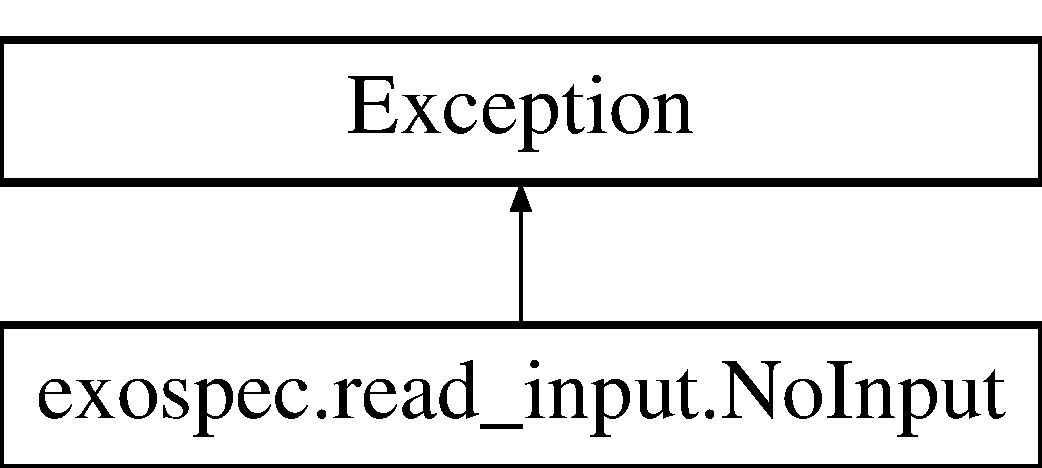
\includegraphics[height=2.000000cm]{classexospec_1_1read__input_1_1_no_input}
\end{center}
\end{figure}


\subsection{Detailed Description}
\begin{DoxyVerb}Raise when no input is found for a parameter\end{DoxyVerb}
 

The documentation for this class was generated from the following file\+:\begin{DoxyCompactItemize}
\item 
/\+Users/heatherp/\+Documents/\+Courses/\+Computational/\+Project/\+Exoplanet\+Spectra/exospec/read\+\_\+input.\+py\end{DoxyCompactItemize}

\hypertarget{classexospec_1_1read__input_1_1read__input}{}\section{exospec.\+read\+\_\+input.\+read\+\_\+input Class Reference}
\label{classexospec_1_1read__input_1_1read__input}\index{exospec.\+read\+\_\+input.\+read\+\_\+input@{exospec.\+read\+\_\+input.\+read\+\_\+input}}


reads the input file and stores the input entries  


\subsection*{Public Member Functions}
\begin{DoxyCompactItemize}
\item 
\mbox{\Hypertarget{classexospec_1_1read__input_1_1read__input_a57a04569bc29445b8bd4f18502b150fe}\label{classexospec_1_1read__input_1_1read__input_a57a04569bc29445b8bd4f18502b150fe}} 
def {\bfseries \+\_\+\+\_\+init\+\_\+\+\_\+} (self, input\+\_\+file)
\item 
def \hyperlink{classexospec_1_1read__input_1_1read__input_a3b21e8723a95f914bb6c329ba68c3d86}{param\+\_\+dic} (self)
\begin{DoxyCompactList}\small\item\em Returns the parameters dictionary. \end{DoxyCompactList}\item 
\mbox{\Hypertarget{classexospec_1_1read__input_1_1read__input_a79332c0dbddf207995b2ad5a602d97ce}\label{classexospec_1_1read__input_1_1read__input_a79332c0dbddf207995b2ad5a602d97ce}} 
def \hyperlink{classexospec_1_1read__input_1_1read__input_a79332c0dbddf207995b2ad5a602d97ce}{is\+\_\+float} (self, string)
\begin{DoxyCompactList}\small\item\em Check if the string contains a float. \end{DoxyCompactList}\end{DoxyCompactItemize}
\subsection*{Public Attributes}
\begin{DoxyCompactItemize}
\item 
\mbox{\Hypertarget{classexospec_1_1read__input_1_1read__input_a3f4c545f0ae322e1a7252a0bf66f3d9f}\label{classexospec_1_1read__input_1_1read__input_a3f4c545f0ae322e1a7252a0bf66f3d9f}} 
{\bfseries param\+\_\+dic}
\end{DoxyCompactItemize}


\subsection{Member Function Documentation}
\mbox{\Hypertarget{classexospec_1_1read__input_1_1read__input_a3b21e8723a95f914bb6c329ba68c3d86}\label{classexospec_1_1read__input_1_1read__input_a3b21e8723a95f914bb6c329ba68c3d86}} 
\index{exospec\+::read\+\_\+input\+::read\+\_\+input@{exospec\+::read\+\_\+input\+::read\+\_\+input}!param\+\_\+dic@{param\+\_\+dic}}
\index{param\+\_\+dic@{param\+\_\+dic}!exospec\+::read\+\_\+input\+::read\+\_\+input@{exospec\+::read\+\_\+input\+::read\+\_\+input}}
\subsubsection{\texorpdfstring{param\+\_\+dic()}{param\_dic()}}
{\footnotesize\ttfamily def exospec.\+read\+\_\+input.\+read\+\_\+input.\+param\+\_\+dic (\begin{DoxyParamCaption}\item[{}]{self }\end{DoxyParamCaption})}

\begin{DoxyReturn}{Returns}
param\+\_\+dic the parameters dictionary 
\end{DoxyReturn}


The documentation for this class was generated from the following file\+:\begin{DoxyCompactItemize}
\item 
/\+Users/heatherp/\+Documents/\+Courses/\+Computational/\+Project/\+Exoplanet\+Spectra/exospec/read\+\_\+input.\+py\end{DoxyCompactItemize}

\hypertarget{classexospec_1_1_transit_model_1_1_transit_model}{}\section{exospec.\+Transit\+Model.\+Transit\+Model Class Reference}
\label{classexospec_1_1_transit_model_1_1_transit_model}\index{exospec.\+Transit\+Model.\+Transit\+Model@{exospec.\+Transit\+Model.\+Transit\+Model}}


Class to estimate the Transit Model with the customized kernel.  


Inheritance diagram for exospec.\+Transit\+Model.\+Transit\+Model\+:\begin{figure}[H]
\begin{center}
\leavevmode
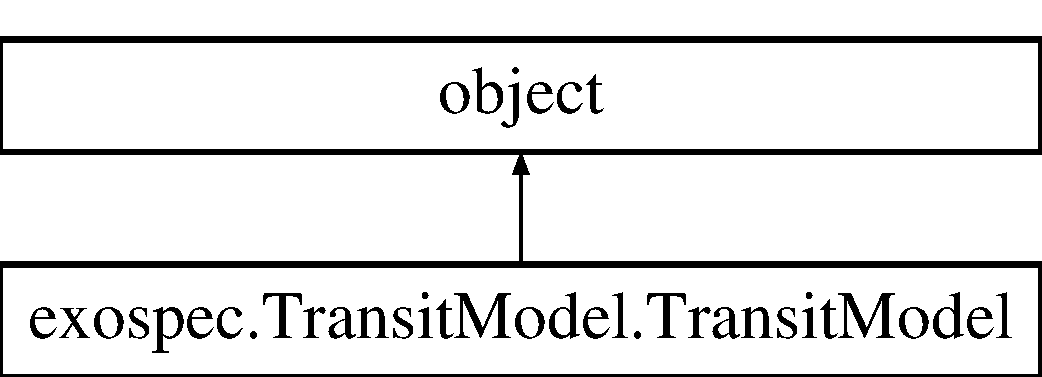
\includegraphics[height=2.000000cm]{classexospec_1_1_transit_model_1_1_transit_model}
\end{center}
\end{figure}
\subsection*{Public Member Functions}
\begin{DoxyCompactItemize}
\item 
def \hyperlink{classexospec_1_1_transit_model_1_1_transit_model_a8e145f1b5965295abcc770f0e72a41b8}{\+\_\+\+\_\+init\+\_\+\+\_\+} (self, kwargs)
\begin{DoxyCompactList}\small\item\em The constructor. \end{DoxyCompactList}\item 
def \hyperlink{classexospec_1_1_transit_model_1_1_transit_model_a1b5933b7cc1aebd32d34beb3df63859a}{set\+\_\+values} (self, dict\+\_\+of\+\_\+values, kwargs)
\begin{DoxyCompactList}\small\item\em Set the parameters of the model based on the values provided. \end{DoxyCompactList}\item 
def \hyperlink{classexospec_1_1_transit_model_1_1_transit_model_ae9e15083b2e989276c67122e8effdc8a}{read\+\_\+limb\+\_\+dark\+\_\+params} (self, kwargs)
\begin{DoxyCompactList}\small\item\em Forms a list of the limb darkening parameters from the user input In case some values are missed, the default ones will be taken. \end{DoxyCompactList}\item 
def \hyperlink{classexospec_1_1_transit_model_1_1_transit_model_a0cc09d939ecb7742b40e33ca870e73ad}{read\+\_\+errors\+\_\+data} (self, kwargs)
\begin{DoxyCompactList}\small\item\em Collects the data about errors that was passed In case some values are missed, the default ones will be taken. \end{DoxyCompactList}\item 
def \hyperlink{classexospec_1_1_transit_model_1_1_transit_model_a282c211d47894b6b9849fd4bd254b696}{update\+\_\+data} (self, time=None, obs=None, kwargs)
\begin{DoxyCompactList}\small\item\em Updates the data for the given parameters. \end{DoxyCompactList}\item 
def \hyperlink{classexospec_1_1_transit_model_1_1_transit_model_a52dd74eef56c0dbb71cb662f684b6182}{update\+\_\+transit\+\_\+params} (self, rp\+\_\+new, u\+\_\+new)
\begin{DoxyCompactList}\small\item\em Updates the parameters of the model. \end{DoxyCompactList}\item 
def \hyperlink{classexospec_1_1_transit_model_1_1_transit_model_a13b851f80d01379553c454f576c79ae5}{update\+\_\+kernel\+\_\+params} (self, a\+\_\+new=None, gamma\+\_\+new=None, variance\+\_\+new=None)
\begin{DoxyCompactList}\small\item\em Updates the hyperparameters of the kernel function. \end{DoxyCompactList}\item 
def \hyperlink{classexospec_1_1_transit_model_1_1_transit_model_abd4eed9477412e6eb684570c3372984b}{update\+Transit\+Mode} (self)
\begin{DoxyCompactList}\small\item\em Updates the transit model parameters. \end{DoxyCompactList}\item 
def \hyperlink{classexospec_1_1_transit_model_1_1_transit_model_abba00977f8fb6ff65f89e2f3e7037ea9}{model} (self)
\begin{DoxyCompactList}\small\item\em Returns the flux values array. \end{DoxyCompactList}\item 
\mbox{\Hypertarget{classexospec_1_1_transit_model_1_1_transit_model_a1a51a8b175518601892d180c83354592}\label{classexospec_1_1_transit_model_1_1_transit_model_a1a51a8b175518601892d180c83354592}} 
def {\bfseries model} (self, params)
\item 
def \hyperlink{classexospec_1_1_transit_model_1_1_transit_model_a4c2121aaf3b3a170e9f0ec0c18911608}{meanfnc} (self, t)
\begin{DoxyCompactList}\small\item\em Mean function for the kernel meaan estimation. \end{DoxyCompactList}\item 
def \hyperlink{classexospec_1_1_transit_model_1_1_transit_model_a4e41db96fc3b1b134bfce74aad263b50}{kernelfnc} (self, x1, x2, p=None)
\begin{DoxyCompactList}\small\item\em Computes the kernel function for the arbitrary sources of errors in the observations. \end{DoxyCompactList}\item 
def \hyperlink{classexospec_1_1_transit_model_1_1_transit_model_a6ff23ea2dfc11348b0ad560c66485be2}{lnlike\+\_\+gp} (self)
\begin{DoxyCompactList}\small\item\em Computes the log likelihood from gaussian process. \end{DoxyCompactList}\item 
def \hyperlink{classexospec_1_1_transit_model_1_1_transit_model_a16ee8da5be7114208af70aa3408615f6}{lnprior\+\_\+base} (self)
\begin{DoxyCompactList}\small\item\em Checks if the batman parameters are within the predefined prior ranges. \end{DoxyCompactList}\item 
def \hyperlink{classexospec_1_1_transit_model_1_1_transit_model_a2c0c838bfee6bdeac30082ebc6cc9517}{lnprior\+\_\+gp} (self)
\begin{DoxyCompactList}\small\item\em Checks if the kernel parameters are within the predefined prior ranges. \end{DoxyCompactList}\item 
def \hyperlink{classexospec_1_1_transit_model_1_1_transit_model_aa791197371e843567a9fdb8565abf154}{lnprob\+\_\+gp} (self)
\begin{DoxyCompactList}\small\item\em Computes the log probability of the parameters for the given data. \end{DoxyCompactList}\item 
def \hyperlink{classexospec_1_1_transit_model_1_1_transit_model_a3a01d6ec61e2e9e95b6d2fd389c0d577}{sample\+\_\+conditional} (self, p, t, y, yerr)
\begin{DoxyCompactList}\small\item\em For a given set of parameters get predicted y values at t, and separate this into the transit signal component and the noise component. \end{DoxyCompactList}\item 
def \hyperlink{classexospec_1_1_transit_model_1_1_transit_model_a11a124a9e7257c0faa6a3577454fa670}{lnprob\+\_\+mcmc} (self, p, t, y, yerr)
\begin{DoxyCompactList}\small\item\em M\+C\+MC A\+PI for the Transit Model object. \end{DoxyCompactList}\end{DoxyCompactItemize}
\subsection*{Public Attributes}
\begin{DoxyCompactItemize}
\item 
\mbox{\Hypertarget{classexospec_1_1_transit_model_1_1_transit_model_a437d43dd1471162d2ee2a3a18c7158d9}\label{classexospec_1_1_transit_model_1_1_transit_model_a437d43dd1471162d2ee2a3a18c7158d9}} 
{\bfseries batman\+\_\+default\+\_\+params}
\item 
\mbox{\Hypertarget{classexospec_1_1_transit_model_1_1_transit_model_a2f80140a13096c5f78fe2d09648f5660}\label{classexospec_1_1_transit_model_1_1_transit_model_a2f80140a13096c5f78fe2d09648f5660}} 
{\bfseries transit\+\_\+default\+\_\+priors}
\item 
\mbox{\Hypertarget{classexospec_1_1_transit_model_1_1_transit_model_ac176c32c71d21399f652496af15213f4}\label{classexospec_1_1_transit_model_1_1_transit_model_ac176c32c71d21399f652496af15213f4}} 
{\bfseries kernel\+\_\+default\+\_\+params}
\item 
\mbox{\Hypertarget{classexospec_1_1_transit_model_1_1_transit_model_a0beb9b7e26c101e5797dc80116612c00}\label{classexospec_1_1_transit_model_1_1_transit_model_a0beb9b7e26c101e5797dc80116612c00}} 
{\bfseries kernel\+\_\+default\+\_\+priors}
\item 
\mbox{\Hypertarget{classexospec_1_1_transit_model_1_1_transit_model_a86c6ecad90c34b29aa1b32350c26e65d}\label{classexospec_1_1_transit_model_1_1_transit_model_a86c6ecad90c34b29aa1b32350c26e65d}} 
{\bfseries data\+\_\+defaults}
\item 
\mbox{\Hypertarget{classexospec_1_1_transit_model_1_1_transit_model_a2e732d47223899b73e671909eb0800d4}\label{classexospec_1_1_transit_model_1_1_transit_model_a2e732d47223899b73e671909eb0800d4}} 
{\bfseries n\+\_\+errors}
\item 
\mbox{\Hypertarget{classexospec_1_1_transit_model_1_1_transit_model_a6a11957fb6cf5302099a3ef97f63b3bd}\label{classexospec_1_1_transit_model_1_1_transit_model_a6a11957fb6cf5302099a3ef97f63b3bd}} 
{\bfseries err\+\_\+names}
\item 
\mbox{\Hypertarget{classexospec_1_1_transit_model_1_1_transit_model_a83d1ba0f875e2b62d22cbfbd79cede25}\label{classexospec_1_1_transit_model_1_1_transit_model_a83d1ba0f875e2b62d22cbfbd79cede25}} 
{\bfseries errors\+\_\+list}
\item 
\mbox{\Hypertarget{classexospec_1_1_transit_model_1_1_transit_model_aa9763ce5105ea17195c2fbe84f6262d1}\label{classexospec_1_1_transit_model_1_1_transit_model_aa9763ce5105ea17195c2fbe84f6262d1}} 
{\bfseries params}
\item 
\mbox{\Hypertarget{classexospec_1_1_transit_model_1_1_transit_model_a8b65c942ed9dcba9fee8b8acbd375cbc}\label{classexospec_1_1_transit_model_1_1_transit_model_a8b65c942ed9dcba9fee8b8acbd375cbc}} 
{\bfseries batman\+\_\+model}
\item 
\mbox{\Hypertarget{classexospec_1_1_transit_model_1_1_transit_model_aa95ce17554f42e897a72baa6e17496d0}\label{classexospec_1_1_transit_model_1_1_transit_model_aa95ce17554f42e897a72baa6e17496d0}} 
{\bfseries model}
\item 
\mbox{\Hypertarget{classexospec_1_1_transit_model_1_1_transit_model_a0e156dc433419b4b8647ad2746427a7c}\label{classexospec_1_1_transit_model_1_1_transit_model_a0e156dc433419b4b8647ad2746427a7c}} 
{\bfseries data\+\_\+dict}
\item 
\mbox{\Hypertarget{classexospec_1_1_transit_model_1_1_transit_model_a6f260ff899915ec7ed640308c05dab5e}\label{classexospec_1_1_transit_model_1_1_transit_model_a6f260ff899915ec7ed640308c05dab5e}} 
{\bfseries model\+\_\+initialized}
\item 
\mbox{\Hypertarget{classexospec_1_1_transit_model_1_1_transit_model_a454db430fc4a7443d3d68d3ef45d6d37}\label{classexospec_1_1_transit_model_1_1_transit_model_a454db430fc4a7443d3d68d3ef45d6d37}} 
{\bfseries kernel\+\_\+type}
\item 
\mbox{\Hypertarget{classexospec_1_1_transit_model_1_1_transit_model_a6b1f393a39f1ab768746334cde5d2a47}\label{classexospec_1_1_transit_model_1_1_transit_model_a6b1f393a39f1ab768746334cde5d2a47}} 
{\bfseries lnprob}
\end{DoxyCompactItemize}


\subsection{Detailed Description}
More details. 

\subsection{Constructor \& Destructor Documentation}
\mbox{\Hypertarget{classexospec_1_1_transit_model_1_1_transit_model_a8e145f1b5965295abcc770f0e72a41b8}\label{classexospec_1_1_transit_model_1_1_transit_model_a8e145f1b5965295abcc770f0e72a41b8}} 
\index{exospec\+::\+Transit\+Model\+::\+Transit\+Model@{exospec\+::\+Transit\+Model\+::\+Transit\+Model}!\+\_\+\+\_\+init\+\_\+\+\_\+@{\+\_\+\+\_\+init\+\_\+\+\_\+}}
\index{\+\_\+\+\_\+init\+\_\+\+\_\+@{\+\_\+\+\_\+init\+\_\+\+\_\+}!exospec\+::\+Transit\+Model\+::\+Transit\+Model@{exospec\+::\+Transit\+Model\+::\+Transit\+Model}}
\subsubsection{\texorpdfstring{\+\_\+\+\_\+init\+\_\+\+\_\+()}{\_\_init\_\_()}}
{\footnotesize\ttfamily def exospec.\+Transit\+Model.\+Transit\+Model.\+\_\+\+\_\+init\+\_\+\+\_\+ (\begin{DoxyParamCaption}\item[{}]{self,  }\item[{}]{kwargs }\end{DoxyParamCaption})}

Takes the disctionary of the parameters and data to customize the object. In case some values are missed, the default one are used. 
\begin{DoxyParams}{Parameters}
{\em self} & The object pointer \\
\hline
{\em $\ast$$\ast$kwargs} & Accepts the dictionary of data, transit and kernel parameters \\
\hline
\end{DoxyParams}


\subsection{Member Function Documentation}
\mbox{\Hypertarget{classexospec_1_1_transit_model_1_1_transit_model_a4e41db96fc3b1b134bfce74aad263b50}\label{classexospec_1_1_transit_model_1_1_transit_model_a4e41db96fc3b1b134bfce74aad263b50}} 
\index{exospec\+::\+Transit\+Model\+::\+Transit\+Model@{exospec\+::\+Transit\+Model\+::\+Transit\+Model}!kernelfnc@{kernelfnc}}
\index{kernelfnc@{kernelfnc}!exospec\+::\+Transit\+Model\+::\+Transit\+Model@{exospec\+::\+Transit\+Model\+::\+Transit\+Model}}
\subsubsection{\texorpdfstring{kernelfnc()}{kernelfnc()}}
{\footnotesize\ttfamily def exospec.\+Transit\+Model.\+Transit\+Model.\+kernelfnc (\begin{DoxyParamCaption}\item[{}]{self,  }\item[{}]{x1,  }\item[{}]{x2,  }\item[{}]{p = {\ttfamily None} }\end{DoxyParamCaption})}


\begin{DoxyParams}{Parameters}
{\em self} & The object pointer \\
\hline
{\em x1} & First time coordinate \\
\hline
{\em x2} & Second time coordinate \\
\hline
{\em p(=\+None)} & Kernel auxiliary parameters \\
\hline
\end{DoxyParams}
\begin{DoxyReturn}{Returns}
Covariance between two points in time 
\end{DoxyReturn}
\mbox{\Hypertarget{classexospec_1_1_transit_model_1_1_transit_model_a6ff23ea2dfc11348b0ad560c66485be2}\label{classexospec_1_1_transit_model_1_1_transit_model_a6ff23ea2dfc11348b0ad560c66485be2}} 
\index{exospec\+::\+Transit\+Model\+::\+Transit\+Model@{exospec\+::\+Transit\+Model\+::\+Transit\+Model}!lnlike\+\_\+gp@{lnlike\+\_\+gp}}
\index{lnlike\+\_\+gp@{lnlike\+\_\+gp}!exospec\+::\+Transit\+Model\+::\+Transit\+Model@{exospec\+::\+Transit\+Model\+::\+Transit\+Model}}
\subsubsection{\texorpdfstring{lnlike\+\_\+gp()}{lnlike\_gp()}}
{\footnotesize\ttfamily def exospec.\+Transit\+Model.\+Transit\+Model.\+lnlike\+\_\+gp (\begin{DoxyParamCaption}\item[{}]{self }\end{DoxyParamCaption})}


\begin{DoxyParams}{Parameters}
{\em self} & The object pointer \\
\hline
\end{DoxyParams}
\begin{DoxyReturn}{Returns}
Log likelihood of a set of observations under the Gaussian process model. 
\end{DoxyReturn}
\mbox{\Hypertarget{classexospec_1_1_transit_model_1_1_transit_model_a16ee8da5be7114208af70aa3408615f6}\label{classexospec_1_1_transit_model_1_1_transit_model_a16ee8da5be7114208af70aa3408615f6}} 
\index{exospec\+::\+Transit\+Model\+::\+Transit\+Model@{exospec\+::\+Transit\+Model\+::\+Transit\+Model}!lnprior\+\_\+base@{lnprior\+\_\+base}}
\index{lnprior\+\_\+base@{lnprior\+\_\+base}!exospec\+::\+Transit\+Model\+::\+Transit\+Model@{exospec\+::\+Transit\+Model\+::\+Transit\+Model}}
\subsubsection{\texorpdfstring{lnprior\+\_\+base()}{lnprior\_base()}}
{\footnotesize\ttfamily def exospec.\+Transit\+Model.\+Transit\+Model.\+lnprior\+\_\+base (\begin{DoxyParamCaption}\item[{}]{self }\end{DoxyParamCaption})}


\begin{DoxyParams}{Parameters}
{\em self} & The object pointer \\
\hline
\end{DoxyParams}
\begin{DoxyReturn}{Returns}
Returns 0 in case transit parameters whithin the prior range and -\/inf otherwise 
\end{DoxyReturn}
\mbox{\Hypertarget{classexospec_1_1_transit_model_1_1_transit_model_a2c0c838bfee6bdeac30082ebc6cc9517}\label{classexospec_1_1_transit_model_1_1_transit_model_a2c0c838bfee6bdeac30082ebc6cc9517}} 
\index{exospec\+::\+Transit\+Model\+::\+Transit\+Model@{exospec\+::\+Transit\+Model\+::\+Transit\+Model}!lnprior\+\_\+gp@{lnprior\+\_\+gp}}
\index{lnprior\+\_\+gp@{lnprior\+\_\+gp}!exospec\+::\+Transit\+Model\+::\+Transit\+Model@{exospec\+::\+Transit\+Model\+::\+Transit\+Model}}
\subsubsection{\texorpdfstring{lnprior\+\_\+gp()}{lnprior\_gp()}}
{\footnotesize\ttfamily def exospec.\+Transit\+Model.\+Transit\+Model.\+lnprior\+\_\+gp (\begin{DoxyParamCaption}\item[{}]{self }\end{DoxyParamCaption})}


\begin{DoxyParams}{Parameters}
{\em self} & The object pointer \\
\hline
\end{DoxyParams}
\begin{DoxyReturn}{Returns}
Returns -\/inf in case parameters out of the range and 0.\+0 if within the prior range 
\end{DoxyReturn}
\mbox{\Hypertarget{classexospec_1_1_transit_model_1_1_transit_model_aa791197371e843567a9fdb8565abf154}\label{classexospec_1_1_transit_model_1_1_transit_model_aa791197371e843567a9fdb8565abf154}} 
\index{exospec\+::\+Transit\+Model\+::\+Transit\+Model@{exospec\+::\+Transit\+Model\+::\+Transit\+Model}!lnprob\+\_\+gp@{lnprob\+\_\+gp}}
\index{lnprob\+\_\+gp@{lnprob\+\_\+gp}!exospec\+::\+Transit\+Model\+::\+Transit\+Model@{exospec\+::\+Transit\+Model\+::\+Transit\+Model}}
\subsubsection{\texorpdfstring{lnprob\+\_\+gp()}{lnprob\_gp()}}
{\footnotesize\ttfamily def exospec.\+Transit\+Model.\+Transit\+Model.\+lnprob\+\_\+gp (\begin{DoxyParamCaption}\item[{}]{self }\end{DoxyParamCaption})}


\begin{DoxyParams}{Parameters}
{\em self} & The object pointer \\
\hline
\end{DoxyParams}
\begin{DoxyReturn}{Returns}
Log probability of the parameters 
\end{DoxyReturn}
\mbox{\Hypertarget{classexospec_1_1_transit_model_1_1_transit_model_a11a124a9e7257c0faa6a3577454fa670}\label{classexospec_1_1_transit_model_1_1_transit_model_a11a124a9e7257c0faa6a3577454fa670}} 
\index{exospec\+::\+Transit\+Model\+::\+Transit\+Model@{exospec\+::\+Transit\+Model\+::\+Transit\+Model}!lnprob\+\_\+mcmc@{lnprob\+\_\+mcmc}}
\index{lnprob\+\_\+mcmc@{lnprob\+\_\+mcmc}!exospec\+::\+Transit\+Model\+::\+Transit\+Model@{exospec\+::\+Transit\+Model\+::\+Transit\+Model}}
\subsubsection{\texorpdfstring{lnprob\+\_\+mcmc()}{lnprob\_mcmc()}}
{\footnotesize\ttfamily def exospec.\+Transit\+Model.\+Transit\+Model.\+lnprob\+\_\+mcmc (\begin{DoxyParamCaption}\item[{}]{self,  }\item[{}]{p,  }\item[{}]{t,  }\item[{}]{y,  }\item[{}]{yerr }\end{DoxyParamCaption})}


\begin{DoxyParams}{Parameters}
{\em self} & The object pointer \\
\hline
{\em p} & Parameters of the transit \\
\hline
{\em t} & Time data \\
\hline
{\em y} & Observations data \\
\hline
{\em yerr} & Errors data \\
\hline
\end{DoxyParams}
\begin{DoxyReturn}{Returns}
Log probability of the chosen parameters 
\end{DoxyReturn}
\mbox{\Hypertarget{classexospec_1_1_transit_model_1_1_transit_model_a4c2121aaf3b3a170e9f0ec0c18911608}\label{classexospec_1_1_transit_model_1_1_transit_model_a4c2121aaf3b3a170e9f0ec0c18911608}} 
\index{exospec\+::\+Transit\+Model\+::\+Transit\+Model@{exospec\+::\+Transit\+Model\+::\+Transit\+Model}!meanfnc@{meanfnc}}
\index{meanfnc@{meanfnc}!exospec\+::\+Transit\+Model\+::\+Transit\+Model@{exospec\+::\+Transit\+Model\+::\+Transit\+Model}}
\subsubsection{\texorpdfstring{meanfnc()}{meanfnc()}}
{\footnotesize\ttfamily def exospec.\+Transit\+Model.\+Transit\+Model.\+meanfnc (\begin{DoxyParamCaption}\item[{}]{self,  }\item[{}]{t }\end{DoxyParamCaption})}


\begin{DoxyParams}{Parameters}
{\em self} & The object pointer \\
\hline
{\em t} & The time data \\
\hline
\end{DoxyParams}
\mbox{\Hypertarget{classexospec_1_1_transit_model_1_1_transit_model_abba00977f8fb6ff65f89e2f3e7037ea9}\label{classexospec_1_1_transit_model_1_1_transit_model_abba00977f8fb6ff65f89e2f3e7037ea9}} 
\index{exospec\+::\+Transit\+Model\+::\+Transit\+Model@{exospec\+::\+Transit\+Model\+::\+Transit\+Model}!model@{model}}
\index{model@{model}!exospec\+::\+Transit\+Model\+::\+Transit\+Model@{exospec\+::\+Transit\+Model\+::\+Transit\+Model}}
\subsubsection{\texorpdfstring{model()}{model()}}
{\footnotesize\ttfamily def exospec.\+Transit\+Model.\+Transit\+Model.\+model (\begin{DoxyParamCaption}\item[{}]{self }\end{DoxyParamCaption})}


\begin{DoxyParams}{Parameters}
{\em self} & The object pointer \\
\hline
\end{DoxyParams}
\begin{DoxyReturn}{Returns}
Model-\/generated observation for the given transit parameters 
\end{DoxyReturn}
\mbox{\Hypertarget{classexospec_1_1_transit_model_1_1_transit_model_a0cc09d939ecb7742b40e33ca870e73ad}\label{classexospec_1_1_transit_model_1_1_transit_model_a0cc09d939ecb7742b40e33ca870e73ad}} 
\index{exospec\+::\+Transit\+Model\+::\+Transit\+Model@{exospec\+::\+Transit\+Model\+::\+Transit\+Model}!read\+\_\+errors\+\_\+data@{read\+\_\+errors\+\_\+data}}
\index{read\+\_\+errors\+\_\+data@{read\+\_\+errors\+\_\+data}!exospec\+::\+Transit\+Model\+::\+Transit\+Model@{exospec\+::\+Transit\+Model\+::\+Transit\+Model}}
\subsubsection{\texorpdfstring{read\+\_\+errors\+\_\+data()}{read\_errors\_data()}}
{\footnotesize\ttfamily def exospec.\+Transit\+Model.\+Transit\+Model.\+read\+\_\+errors\+\_\+data (\begin{DoxyParamCaption}\item[{}]{self,  }\item[{}]{kwargs }\end{DoxyParamCaption})}


\begin{DoxyParams}{Parameters}
{\em self} & The object pointer \\
\hline
{\em $\ast$$\ast$kwargs} & Dictionary of the parameters to pass \\
\hline
\end{DoxyParams}
\mbox{\Hypertarget{classexospec_1_1_transit_model_1_1_transit_model_ae9e15083b2e989276c67122e8effdc8a}\label{classexospec_1_1_transit_model_1_1_transit_model_ae9e15083b2e989276c67122e8effdc8a}} 
\index{exospec\+::\+Transit\+Model\+::\+Transit\+Model@{exospec\+::\+Transit\+Model\+::\+Transit\+Model}!read\+\_\+limb\+\_\+dark\+\_\+params@{read\+\_\+limb\+\_\+dark\+\_\+params}}
\index{read\+\_\+limb\+\_\+dark\+\_\+params@{read\+\_\+limb\+\_\+dark\+\_\+params}!exospec\+::\+Transit\+Model\+::\+Transit\+Model@{exospec\+::\+Transit\+Model\+::\+Transit\+Model}}
\subsubsection{\texorpdfstring{read\+\_\+limb\+\_\+dark\+\_\+params()}{read\_limb\_dark\_params()}}
{\footnotesize\ttfamily def exospec.\+Transit\+Model.\+Transit\+Model.\+read\+\_\+limb\+\_\+dark\+\_\+params (\begin{DoxyParamCaption}\item[{}]{self,  }\item[{}]{kwargs }\end{DoxyParamCaption})}


\begin{DoxyParams}{Parameters}
{\em self} & The object pointer \\
\hline
{\em $\ast$$\ast$kwargs} & Dictionary of the parameters to pass \\
\hline
\end{DoxyParams}
\mbox{\Hypertarget{classexospec_1_1_transit_model_1_1_transit_model_a3a01d6ec61e2e9e95b6d2fd389c0d577}\label{classexospec_1_1_transit_model_1_1_transit_model_a3a01d6ec61e2e9e95b6d2fd389c0d577}} 
\index{exospec\+::\+Transit\+Model\+::\+Transit\+Model@{exospec\+::\+Transit\+Model\+::\+Transit\+Model}!sample\+\_\+conditional@{sample\+\_\+conditional}}
\index{sample\+\_\+conditional@{sample\+\_\+conditional}!exospec\+::\+Transit\+Model\+::\+Transit\+Model@{exospec\+::\+Transit\+Model\+::\+Transit\+Model}}
\subsubsection{\texorpdfstring{sample\+\_\+conditional()}{sample\_conditional()}}
{\footnotesize\ttfamily def exospec.\+Transit\+Model.\+Transit\+Model.\+sample\+\_\+conditional (\begin{DoxyParamCaption}\item[{}]{self,  }\item[{}]{p,  }\item[{}]{t,  }\item[{}]{y,  }\item[{}]{yerr }\end{DoxyParamCaption})}


\begin{DoxyParams}{Parameters}
{\em self} & The object pointer \\
\hline
{\em p} & Parameters of the transit \\
\hline
{\em t} & Time data \\
\hline
{\em y} & Observations data \\
\hline
{\em yerr} & Errors data \\
\hline
\end{DoxyParams}
\begin{DoxyReturn}{Returns}
Predicted observations 
\end{DoxyReturn}
\mbox{\Hypertarget{classexospec_1_1_transit_model_1_1_transit_model_a1b5933b7cc1aebd32d34beb3df63859a}\label{classexospec_1_1_transit_model_1_1_transit_model_a1b5933b7cc1aebd32d34beb3df63859a}} 
\index{exospec\+::\+Transit\+Model\+::\+Transit\+Model@{exospec\+::\+Transit\+Model\+::\+Transit\+Model}!set\+\_\+values@{set\+\_\+values}}
\index{set\+\_\+values@{set\+\_\+values}!exospec\+::\+Transit\+Model\+::\+Transit\+Model@{exospec\+::\+Transit\+Model\+::\+Transit\+Model}}
\subsubsection{\texorpdfstring{set\+\_\+values()}{set\_values()}}
{\footnotesize\ttfamily def exospec.\+Transit\+Model.\+Transit\+Model.\+set\+\_\+values (\begin{DoxyParamCaption}\item[{}]{self,  }\item[{}]{dict\+\_\+of\+\_\+values,  }\item[{}]{kwargs }\end{DoxyParamCaption})}

In case some values are missed, the default ones will be taken. 
\begin{DoxyParams}{Parameters}
{\em self} & The object pointer \\
\hline
{\em dict\+\_\+of\+\_\+values} & Dictionary of the parameters to pass \\
\hline
\end{DoxyParams}
\mbox{\Hypertarget{classexospec_1_1_transit_model_1_1_transit_model_a282c211d47894b6b9849fd4bd254b696}\label{classexospec_1_1_transit_model_1_1_transit_model_a282c211d47894b6b9849fd4bd254b696}} 
\index{exospec\+::\+Transit\+Model\+::\+Transit\+Model@{exospec\+::\+Transit\+Model\+::\+Transit\+Model}!update\+\_\+data@{update\+\_\+data}}
\index{update\+\_\+data@{update\+\_\+data}!exospec\+::\+Transit\+Model\+::\+Transit\+Model@{exospec\+::\+Transit\+Model\+::\+Transit\+Model}}
\subsubsection{\texorpdfstring{update\+\_\+data()}{update\_data()}}
{\footnotesize\ttfamily def exospec.\+Transit\+Model.\+Transit\+Model.\+update\+\_\+data (\begin{DoxyParamCaption}\item[{}]{self,  }\item[{}]{time = {\ttfamily None},  }\item[{}]{obs = {\ttfamily None},  }\item[{}]{kwargs }\end{DoxyParamCaption})}


\begin{DoxyParams}{Parameters}
{\em self} & The object pointer \\
\hline
{\em time(=\+None)} & Time data \\
\hline
{\em obs(=\+None)} & Observations data \\
\hline
{\em $\ast$$\ast$kwargs} & Handles arbitrary number of the errors that was passed \\
\hline
\end{DoxyParams}
\mbox{\Hypertarget{classexospec_1_1_transit_model_1_1_transit_model_a13b851f80d01379553c454f576c79ae5}\label{classexospec_1_1_transit_model_1_1_transit_model_a13b851f80d01379553c454f576c79ae5}} 
\index{exospec\+::\+Transit\+Model\+::\+Transit\+Model@{exospec\+::\+Transit\+Model\+::\+Transit\+Model}!update\+\_\+kernel\+\_\+params@{update\+\_\+kernel\+\_\+params}}
\index{update\+\_\+kernel\+\_\+params@{update\+\_\+kernel\+\_\+params}!exospec\+::\+Transit\+Model\+::\+Transit\+Model@{exospec\+::\+Transit\+Model\+::\+Transit\+Model}}
\subsubsection{\texorpdfstring{update\+\_\+kernel\+\_\+params()}{update\_kernel\_params()}}
{\footnotesize\ttfamily def exospec.\+Transit\+Model.\+Transit\+Model.\+update\+\_\+kernel\+\_\+params (\begin{DoxyParamCaption}\item[{}]{self,  }\item[{}]{a\+\_\+new = {\ttfamily None},  }\item[{}]{gamma\+\_\+new = {\ttfamily None},  }\item[{}]{variance\+\_\+new = {\ttfamily None} }\end{DoxyParamCaption})}


\begin{DoxyParams}{Parameters}
{\em self} & The object pointer \\
\hline
{\em a\+\_\+new} & New value of the kernel\+\_\+a \\
\hline
{\em gamma\+\_\+new} & New value of the kernel\+\_\+gamma \\
\hline
\end{DoxyParams}
\mbox{\Hypertarget{classexospec_1_1_transit_model_1_1_transit_model_a52dd74eef56c0dbb71cb662f684b6182}\label{classexospec_1_1_transit_model_1_1_transit_model_a52dd74eef56c0dbb71cb662f684b6182}} 
\index{exospec\+::\+Transit\+Model\+::\+Transit\+Model@{exospec\+::\+Transit\+Model\+::\+Transit\+Model}!update\+\_\+transit\+\_\+params@{update\+\_\+transit\+\_\+params}}
\index{update\+\_\+transit\+\_\+params@{update\+\_\+transit\+\_\+params}!exospec\+::\+Transit\+Model\+::\+Transit\+Model@{exospec\+::\+Transit\+Model\+::\+Transit\+Model}}
\subsubsection{\texorpdfstring{update\+\_\+transit\+\_\+params()}{update\_transit\_params()}}
{\footnotesize\ttfamily def exospec.\+Transit\+Model.\+Transit\+Model.\+update\+\_\+transit\+\_\+params (\begin{DoxyParamCaption}\item[{}]{self,  }\item[{}]{rp\+\_\+new,  }\item[{}]{u\+\_\+new }\end{DoxyParamCaption})}


\begin{DoxyParams}{Parameters}
{\em self} & The object pointer \\
\hline
{\em rp\+\_\+new} & New value of the rp parameter \\
\hline
{\em u\+\_\+new} & New list of values for the limb darkening \\
\hline
\end{DoxyParams}
\mbox{\Hypertarget{classexospec_1_1_transit_model_1_1_transit_model_abd4eed9477412e6eb684570c3372984b}\label{classexospec_1_1_transit_model_1_1_transit_model_abd4eed9477412e6eb684570c3372984b}} 
\index{exospec\+::\+Transit\+Model\+::\+Transit\+Model@{exospec\+::\+Transit\+Model\+::\+Transit\+Model}!update\+Transit\+Mode@{update\+Transit\+Mode}}
\index{update\+Transit\+Mode@{update\+Transit\+Mode}!exospec\+::\+Transit\+Model\+::\+Transit\+Model@{exospec\+::\+Transit\+Model\+::\+Transit\+Model}}
\subsubsection{\texorpdfstring{update\+Transit\+Mode()}{updateTransitMode()}}
{\footnotesize\ttfamily def exospec.\+Transit\+Model.\+Transit\+Model.\+update\+Transit\+Mode (\begin{DoxyParamCaption}\item[{}]{self }\end{DoxyParamCaption})}


\begin{DoxyParams}{Parameters}
{\em self} & The object pointer \\
\hline
\end{DoxyParams}


The documentation for this class was generated from the following file\+:\begin{DoxyCompactItemize}
\item 
Transit\+Model.\+py\end{DoxyCompactItemize}

%--- End generated contents ---

% Index
\backmatter
\newpage
\phantomsection
\clearemptydoublepage
\addcontentsline{toc}{chapter}{Index}
\printindex

\end{document}
